
% Ricardo Rocha, January 21, 2013

%\documentclass[times,10pt,twocolumn]{article} 
%\usepackage{latex8}
%\usepackage{times}

%\documentclass[10pt]{IEEEtran}
\documentclass[conference]{IEEEtran}
% allow \thanks
\IEEEoverridecommandlockouts

\usepackage[pdftex]{graphicx}
%%\usepackage{epsf}
\usepackage[tight,footnotesize]{subfigure}
%%\usepackage{multirow}
%%\usepackage{tabularx}
%\usepackage{setspace}
\usepackage[ruled,linesnumbered]{algorithm2e}
%%\usepackage{algorithm2e}
\usepackage{amsmath}
%\usepackage{fullpage}


% very commonly used defs and commands

% packages needed for THESE DEFS

\usepackage[usenames,dvipsnames]{color}
\usepackage{amsfonts}
\usepackage{epigraph}


% General
\newcommand{\tab}{\hspace{0.7cm}}
\newcommand{\REM}[1]{}  
\newcommand{\ti}[1]{\textsf{#1}}
\def\descWidth{3in}


% Abbreviations
\def\eg{{\it e.g.}}
\def\ie{{\it i.e.}}
\def\etal{{\it et~al.}}
\def\etc{{\it etc.}}
\def\viz{{\it viz.}}
\def\bwu{{\tt bwu}}

% center a single cell of a table
\newcommand{\cc}[1]{\multicolumn{1}{c}{#1}}
\newcommand{\ccb}[1]{\multicolumn{1}{c}{\bf #1}}
\newcommand{\mc}[3]{\multicolumn{#1}{#2}{#3}}
\newcommand{\mccb}[2]{\multicolumn{#1}{c}{\bf #2}}
% extra top/bottom row spacing.  must be *in* a cell on the row
\def\T{\rule{0pt}{2.1ex}}
\def\B{\rule[-1.2ex]{0pt}{0pt}}


% Math
%\newcommand{\vect}[1]{\ensuremath{\vec{#1}}}
\newcommand{\vect}[1]{\ensuremath{\mathbf{#1}}}
\newcommand{\pair}[2]{\ensuremath{\langle #1, #2 \rangle}}
\newcommand{\range}[2]{\ensuremath{\left[#1, #2\right]}}
\newcommand{\rangeC}[2]{\ensuremath{\left[#1,&#2\right]}}
\newcommand{\floor}[1]{\ensuremath{\left\lfloor #1 \right\rfloor}}
\newcommand{\ceil}[1]{\ensuremath{\left\lceil #1 \right\rceil}}
%\newcommand{\blt}[1]{\ensuremath{t_\emptyset}(#1)}
\def\ntau{\ensuremath{\tau^{\scalebox{0.5}[1.0]{\(-\)}1}}}

% - sets
\newcommand{\fancy}[1]{\ensuremath{\mathcal{#1}}}
\newcommand{\set}[2]{\ensuremath{\mathcal{#1}=\{#2\}}}
\newcommand{\sset}[2]{\ensuremath{#1=\{#2\}}}

% - statistics
\def\V{\mathbb{V}}
\def\E{\mathbb{E}}
\def\P{\mathbb{P}}
\def\dep{\ensuremath{\amalg}}
\def\indep{\ensureath{\not\propto}} % This is not the symbol used in AllStat...


% Names
\def\bzip{{\tt bzip2}}
\def\crafty{{\tt crafty}}
\def\gap{{\tt GAP}}
\def\gzip{{\tt gzip}}
\def\mcf{{\tt mcf}}
\def\parser{{\tt parser}}
\def\vpr{{\tt vpr}}
\def\gobmk{{\tt gobmk}}
\def\gcc{{\tt gcc}}
\def\lbm{{\tt LBM}}
\def\mesa{{\tt mesa}}
\def\twolf{{\tt twolf}}

\def\Bzip{{\tt Bzip2}}
\def\Crafty{{\tt Crafty}}
\def\Gap{{\tt GAP}}
\def\Gzip{{\tt Gzip}}
\def\Mcf{{\tt Mcf}}
\def\Parser{{\tt Parser}}
\def\Vpr{{\tt Vpr}}
\def\Gobmk{{\tt Gobmk}}
\def\Gcc{{\tt Gcc}}
\def\Lbm{{\tt LBM}}
\def\Mesa{{\tt Mesa}}
\def\Twolf{{\tt Twolf}}

\def\Wfull{{\ifColorText{Red}{\fancy{W}}}}


% Colored stuff; Comments and References

% Colors on or off: Pick ONE
\newcommand{\ifColorText}[2]{\textcolor{#1}{#2}}  % Colors ON
%\newcommand{\ifColorText}[2]{{#2}}                % Colors OFF

% Comments on or off: Pick ONE
\newcommand{\ifComments}[1]{{#1}}                 % Comments ON
%\newcommand{\ifComments}[1]{\REM{#1}}             % Comments OFF

\def\CProf{\ifColorText{Green}{CProf}}
\newcommand{\funcname}[2][RoyalBlue]{\ifColorText{#1}{\ensuremath{\mathsf{#2}}}}
\newcommand{\name}[1]{{\tt #1}}
\newcommand{\iname}[1]{\ensuremath{\mathsf{#1}}}
\newcommand{\funcOf}[3][RoyalBlue]{\funcname[#1]{#2(}{#3}\funcname[#1]{)}}

\def\Benefit{\funcname{Benefit}}
\newcommand{\BenefitOf}[1]{\funcOf{Benefit}{#1}}

\def\Cost{\funcname{Cost}}
\newcommand{\CostOf}[1]{\funcOf{Cost}{#1}}

\def\Reward{\funcname{Reward}}
\newcommand{\RewardOf}[1]{\funcOf{Reward}{#1}}

\def\Score{\funcname{Score}}
\newcommand{\ScoreOf}[1]{\funcOf{Score}{#1}}

\newcommand{\am}[1]{\ifComments{\noindent\textcolor{red}{Nelson: {#1}}}}
\newcommand{\pb}[1]{\ifComments{\noindent\textcolor{brown}{Paul: {#1}}}}
\newcommand{\rr}[1]{\ifComments{\noindent\textcolor{blue}{Rocha: {#1}}}}
\newcommand{\br}[1]{\ifComments{\noindent\textcolor{green}{Bruno: {#1}}}}

\newcommand{\newT}[1]{\ifColorText{red}{{\ifComments{\tiny [ed]} #1}}}
\newcommand{\HL}[1]{\ifColorText{BurntOrange}{\ifComments{\tiny [chk]} #1}}
\newcommand{\RW}[1]{\ifColorText{CarnationPink}{\ifComments{\tiny [redo]} #1}}

% modification for anonimity in double-blind reviewing
% Parameter 1 is original text, parameter 2 is replacement text
\newcommand{\doubleblind}[2]{#2}

%-- Reference Chapter
\newcommand{\refChapter}[1]{\ifColorText{blue}{Chapter~\ref{#1}}}
%\newcommand{\refChapter}[1]{Chapter~\ref{#1}}

%-- Reference Section
\newcommand{\refSection}[1]{\ifColorText{Green}{Section~\ref{#1}}}
%\newcommand{\refSection}[1]{\textcolor{green}{{\S}\ref{#1}}}
%\newcommand{\refSection}[1]{Section~\ref{#1}}
%\newcommand{\refSection}[1]{{\S}\ref{#1}}

%-- Reference Table
\newcommand{\refTable}[1]{\ifColorText{Plum}{Table~\ref{#1}}}
%\newcommand{\refTable}[1]{Table~\ref{#1}}

%-- Reference Figure
\newcommand{\refFigure}[1]{\ifColorText{Red}{Figure~\ref{#1}}}
%\newcommand{\refFigure}[1]{Figure~\ref{#1}}

%-- Reference Figure
\newcommand{\refAlgorithm}[1]{\ifColorText{Turquoise}{Algorithm~\ref{#1}}}
%\newcommand{\refAlgorithm}[1]{Algorithm~\ref{#1}}

%-- Reference Figure
\newcommand{\refEqn}[1]{\ifColorText{Turquoise}{Equation~\ref{#1}}}
%\newcommand{\refEqn}[1]{Equation~\ref{#1}}

%-- Reference Line (of algorithm, by label)
\newcommand{\refLine}[1]{\ifColorText{Turquoise}{line~\ref{#1}}}


%\pagestyle{empty}
\pagestyle{plain}


% Colors on or off: Pick ONE
\renewcommand{\ifColorText}[2]{\textcolor{#1}{#2}}  % Colors ON
%\renewcommand{\ifColorText}[2]{{#2}}                % Colors OFF

% Comments on or off: Pick ONE
\renewcommand{\ifComments}[1]{{#1}}                 % Comments ON
%\renewcommand{\ifComments}[1]{\REM{#1}}             % Comments OFF


\newcommand{\abbrev}[2][Blue]{\ifColorText{#1}{\ensuremath{\mathrm{#2}}}}

\def\llvm{{\ifColorText{Red}{{\tt LLVM}}}}
\def\PP{{\ifColorText{Orange}{PP}}}
\def\CP{{\ifColorText{RoyalBlue}{CP}}}
\def\CEP{{\ifColorText{RoyalBlue}{CEP}}}
\def\CPP{{\ifColorText{RoyalBlue}{CPP}}}
\def\HN{{\ifColorText{OliveGreen}{HN}}}
\def\CG{{\ifColorText{Periwinkle}{CG}}}
\def\CFG{{\ifColorText{Fuchsia}{CFG}}}
\def\FDO{{\ifColorText{Magenta}{FDO}}}
\def\DF{{\ifColorText{Blue}{\ensuremath{\mathrm{DF}}}}}
\def\FDI{{\ifColorText{Magenta}{FDI}}}
\def\CS{\abbrev{CS}}

\newcommand{\DFact}[2]{{\ifColorText{Blue}{\ensuremath{\mathrm{\DF}_{{#1}\rightarrow {#2}}}}}}


\begin{document}
\thispagestyle{empty}

\title{An Empirical Evaluation of Combined Profiling}

%\pagenumbering{arabic}

%\authorinfo{\ }{\ }{\ }
\author{\IEEEauthorblockN{Ricardo Luis de Azevedo da Rocha\thanks{This research was done while the nth author was in a sabbatical year at the University of Alberta, supported by grant 2011/17096-5 from the Funda\c{c}\~{a}o de Amparo \`{a} Pesquisa do Estado de S\~{a}o Paulo -- FAPESP.}}
\IEEEauthorblockA{Dept. of Computing Engineering\\
University of Sao Paulo and \\ Dept. of Computing Science \\ University of Alberta\\
Edmonton, Alberta, T6G 2E8, Canada\\
Email: rlarocha@usp.br\\ \hspace{53pt}azevedod@ualberta.ca}
\and
\IEEEauthorblockN{Paul Berube}
\IEEEauthorblockA{Dept. of Computing Science\\
University of Alberta\\
Edmonton, Alberta, T6G 2E8, Canada\\
Email: pberube@ualberta.ca}
\and
\IEEEauthorblockN{Bruno Rosa}
\IEEEauthorblockA{Dept. of Computing Science\\
University of Alberta\\
Edmonton, Alberta, T6G 2E8, Canada\\
Email: brosa@ualberta.ca}
\and
\IEEEauthorblockN{Jos\'{e} Nelson Amaral\thanks{This research is supported by fellowships and grants from the Natural Sciences and Engineering Research Council of Canada (NSERC), the Informatics Circle of Research Excellence (iCORE), and the Canadian Foundation for innovation (CFI).}}
\IEEEauthorblockA{Dept. of Computing Science\\
University of Alberta\\
Edmonton, Alberta, T6G 2E8, Canada\\
Email: amaral@cs.ualberta.ca}}


\maketitle

\rr{Title is not set, just to fill in the blank; The order of the authors is meaningless now}
\begin{abstract}

A common practice used to evaluate Feedback Directed Optimization
(\FDO) code transformations is to perform a single-run profile to characterize the behaviour of a program and then to evaluate the performance
of the FDO transformation using  a single-input run of the program. This research addresses this shortcoming of FDO research using a new methodology, the {\em combined profiling} (\CP), to both inform the FDO decisions and produce a more significant performance evaluation of the code produced with FDO. Combined profiling can be applied to many different
optimization techniques, in this paper  we apply it to inlining, a simple and general technique
that allows many other optimization techniques to be performed afterwards. Besides the application of combining profiling and a proper evaluation of inlining, this work also investigates better strategies for inlining and searches for and
better parameter values for the inlining heuristics. The main finds are....

%This paper assesses {\em combined profiling} (CP): a practical
%methodology to produce statistically sound combined profiles from
%multiple runs of a program.  Combining profiles is often necessary to
%properly characterize the behavior of a program to support
%Feedback-Directed Optimization (FDO).  Previous publications described
%the \CP\ methodology, hence the approach here is to evaluate how to
%improve the compiler system parameters and algorithms.  The parameters
%were tuned in, and the choices made by the main algorithm, defining which
%functions were to be inlined, was assessed by comparing its outcome with
%random choices.  A slight change to the algorithm was also empirically
%evaluated trying to improve its result by introducing a knapsack view
%of the problem. The compiler system and the \CP\ methodology were
%evaluated in \llvm\ using SPEC CPU 2006 benchmarks.

%\CP\ models program behaviors
%over multiple runs by estimating their empirical distributions,
%providing the inferential power of probability distributions to code
%transformations.  These distributions are build from traditional
%single-run point profiles; no new profiling infrastructure is
%required.  The small fixed size of this data representation keeps
%profile sizes, and the computational costs of profile queries,
%independent of the number of profiles combined.  However, when using
%even a single program run, a \CP\ maintains the information available
%in the point profile, allowing \CP\ to be used as a drop-in
%replacement for existing techniques. The quality of the information
%generated by the \CP\ methodology is evaluated in \llvm\ using SPEC
%CPU 2006 benchmarks.

\end{abstract}

\section{Introduction}
	\label{sec:intro}
	\rr{
Purpose of the research:
\begin{enumerate}
\item Conduct experiments to study the current status of Combined profiling applied to inlining.
\item Compare the results produced using the methodology with traditional approaches. (here we have to compare the results with the single run experiment) Probably this is the last experiment to be tried.
\item Verify if the profiling makes any difference or not - by means of a random choice of functions to inline.
\item Tune in the constant values of the system.
\item Define which strategy it more appropriate to use in this approach to inlining, simple sort, or a more sophisticated choice, based on the knapsack problem.
\end{enumerate}
}

%I guess this is it ...

%=====================

For most useful programs, the program's behaviour during execution depends on the program's input.
Consequently, there is seldom an optimally-efficient executable
representation of high-level source code that executes
in the least possible amount of time for every program input.  Even
given an optimization criteria, such as processing throughput, and a
reasonable set of program inputs, creating an executable whose
performance is optimal for that set of inputs is (provably)
intractable. Moreover, it is infeasible to approach compiler design as
a single problem.  Instead, compilers apply a series of {\it
transformations} that attempt to improve
the efficiency of a particular region of code in a specific way.  For
instance, ~\ref{sec:inlining} presents a function-inlining
transformation that replaces a function call by a copy of the body of
the called function. This transformation improves program efficiency
by eliminating the overhead of making function calls, while improving
the effectiveness of subsequent transformations.

Research in compiler transformations often demonstrates heroic efforts
in both the identification and abstract analysis of opportunities to
improve program efficiency, and in the concrete implementation of
these ideas.  However, standard practices at the evaluation stage of
the scientific process are modest at best, perhaps because code
transformations have a long history of providing significant benefits
in practical, every-day situations.  In most cases, compilers are
evaluated using a collection of programs, with each program evaluated
using a timing run on a single evaluation input.  The deficiencies of
this evaluation process are particularly prevalent, and especially
disconcerting, when {\it feedback-directed optimization} (\FDO) is
used to guide a transformation.  In this scenario, instrumentation is
inserted into the program during an initial compilation in order to
collect a profile of the run-time behaviour of the program during one
or more training runs.  The profile is used in a second compilation of
the program to help the compiler assess the benefit of code
transformation opportunities.  The current standard practice for
evaluating an \FDO\ compiler uses the profile of a single-training
input to guide transformations, and evaluates the transformed program
with a single evaluation input.  These standard practices set program
inputs as controlled variables.  However, performance evaluation
should be generalizable to real-world program workloads.
Consequently, the program-input dimensions of a rigorous evaluation of
compiler performance must be manipulated variables.

Performance evaluation is a challenging, multi-faceted problem.  In
this research, performance is always assessed in terms of program
execution time\footnote{Other measures of performance include power
consumption and code size.}  One dimension of this challenge is the
choice between evaluating throughput or latency.  Given a collection of tasks
(\eg, the programs in a benchmark suite or runs of a single program on
a workload of inputs), throughput measures the total time required to
complete all tasks sequentially.  Conversely, latency considers the
tasks in parallel and measures the task that takes the longest.
Improving throughput means reducing average execution time; improving
latency means reducing worst-case execution time.  Both types of
performance are important, and both approaches to evaluation are
valid. Fortunately, shifting focus is often as simple as changing the
weighting used to combine measurements from the individual tasks.
Different aspects of this work assume different performance goals and
thus perform the weighting in different ways.  Consider each of these
approaches as one possible option for evaluation, independent of the
specific evaluation in which they appear.  A real-world application of
any of the ideas presented here will have unique performance goals,
and can mix-and-match these approaches as appropriate.

Previous work has not addressed the problem of representing and
utilizing multi-run profiles.  An \FDO\ compiler should not simply add
or average profiles from multiple runs, because such a profile does
not provide any information about the variations in program behaviors
observed between different inputs. ~\cite{BerubePhD} uses {\it
Combined Profiling} (\CP) to merge the profiles from multiple runs
into a distribution model that allows code transformations to consider
cross-run behavior variations.  Experimental results demonstrate that
meaningful behavior variation is present in the program workloads,
and that this variation is successfully captured and represented by
the \CP\ methodology.

%=====================

This research uses a different approach and its goal is to assess the results
of {\em combined profiling} (\CP). There have been some recent efforts trying
to apply multiple profiles to \FDO\, and also to evaluate the performance of a
program from multiple inputs. \CP\ can be applied to many different optimization
techniques, such as inlining, loop unrolling, etc. We decided to apply \CP\ to
inlining, because it allows many other optimization techniques to be performed
afterwards.

%=====================

The \FDO-based inliner presented in ~\cite{BerubePhD}
demonstrates how a transformation can use the information stored in a
combined profile. The feedback-directed inlining framework sorts
inlining opportunities according to parameterized reward functions that
query a combined profile using distribution
quantiles.  These components are brought together by
performing a thorough cross-validated evaluation of the \CP-informed
inliner.

%=====================

Proceeding with our research, we were challenged to define strategies for the
inliner, and also to search for better parameter values for it. But we know that
this set is not suited to all benchmarks, as reported in Kulkarni \etal \cite{KulkarniCGO13}.
To address the former problem we defined three different algorithms to choose a good candidate for inlining.
One acting as a best-search at each execution step, another that defines a set of
better candidates in a knapsack fashion. The last one performs a random choice
which allowed us to effectively compare our results for the strategy.

For the problem of defining the best set point for the parameters, we decided to employ
a Machine Learning technique in order to define a "sweet spot". This part of our research
searched for a technique that could operate on limited data and unknown optimization
space. The behavior of the optimization technique had to be steady in any space, because
we didn't know whether the space of parameters is convex, or differentiable. And we could
not afford to have many values for the parameter set. We decided to use the Simulated
Annealing, or the SPSA - Simultaneous Perturbation Stochastic Approximation, because
both techniques can deal with our constraints.

%This paper shows our results on evaluating \CP\ and the application
%case for inlining.

%Although the usual way to do research in Feedback Directed Optimization
%is to perform a single-run input training and single data testing, recently
%are being developed other approaches to this problem. The main goal of
%these new approaches is to perform multiple-runs under multiple data, because
%some questions concerning the single-run approach arose, such as, is this
%method accurate, or proper, or reliable?

%In an attempt to answer to these questions the  {\it Combined Profiling} (\CP) 
%methodology \cite{BerubePhD} was proposed.

%CP can be used to assess many different compiling techniques, but we chose to
%apply this methodology to study inlining.

%The inlining technique enables series of transformations and

%One of the problems with inlining is the parameter tuning, and choosing inlining strategies.

%We're doing this for the first time using multiple data and multiple runs..

%Our approach is to use an empirical validation of the CP process for the inlining case.

%=====================

Several open questions about the use of profiles collected from
multiple runs of a program were addressed and assessed in \cite{BerubeISPASS12}.
Now there are still some questions, as multiple profiles are
combined. What is the impact of \CP\ in a controlled case study?
\FDO\ decisions can be more accurate using \CP\ instead of single-run evaluation?
How the parameters can be tuned in? Which strategy to be used, considering
FDO?

This paper addresses these questions by using an empirical validation of the \CP\ process
for the inlining case. At first by arguing that the behavior variations in an application due
to multiple inputs produces better \FDO\ decisions.  It also argues that the parameters can be
tuned in using machine learning techniques. As already mentioned the case proposed was
for inlining, and we compared the choice of candidate to inline using the best candidate of a
sorted list with random choice, and with a more sophisticated choice, based on the knapsack
problem. The application of \CP\ to other situations with multiple profiling instances, such as
profiling program phases individually, is not within the scope of this paper.

The main contribution of this paper are:
\begin{itemize}
\item {\it Assessment of combined profiling} (\CP), is performed using
  the case of {\it inlining} and the behavior of single-runs and \CP-runs
  are analyzed (Section~\ref{sec:results}).

\item {\it Parameter tuning}, is done by a machine learning algorithm to find the 
  sweetspot for a set of inlining parameters (Section~\ref{sec:ml}).

\item {\it Inline candidates} can be chosen in many different ways, so
  analyzing behavior variability for random choice, simple sort and
  a version of the knapsack problem shed light to this problem (Section~\ref{sec:choice}).

\end{itemize}



\section{Combined Profiling}
	\label{sec:cmbprof}
	

Capturing behavior variations across inputs is important in the design
of an \FDO\ compiler. A number of speculative code transformations are
known to benefit from \FDO, including speculative partial redundancy
elimination~\cite{ChowChanPLDI97,GuptaICCL98}, trace-based
scheduling and others~\cite{BodikGuptaPLDI97,ChekuriMICRO96}.% Several
%open questions remain about the use of profiles collected from
%multiple runs of a program.  How should the multiple profiles be
%combined? Is it sufficient to simply average the multiple
%measurements? Is it necessary to compute the parameters for an assumed
%statistical distribution of the measurements? Or is there a simple
%technique to combine the measurements and provide useful statistics to
%\FDO?

This section argues that the behavior
variations in an application due to multiple inputs should be
evaluated by \FDO\ decisions.  It also argues that a full parametric
estimation of a statistical distribution is not only unnecessary, but
it may also mislead FDO decisions if the wrong distribution is assumed
or there is insufficient data to accurately estimate the
parameters.% Instead, it proposes the use of a non-parametric empirical
%distribution that makes no assumptions about the shape of the actual
%distribution. 


A major challenge in the use of traditional single-training-run \FDO\
is the selection of a profiling data input that is representative of
the execution of the program throughout its lifetime.  For large and
complex programs dealing with many use cases and used by a multitude
of users, assembling an appropriately representative workload may be a
difficult task.  Picking a solitary training run to represent such a
space is far more challenging, or potentially impossible, if use-cases
are mutually-exclusive.  While benchmark programs can be modified to
combine such use-cases into a single run, %(\refSection{single:spec}),
this approach is obviously inapplicable to real programs.  Moreover,
user workloads are prone to change over time.  Ensuring stable
performance across all inputs in today's workload prevents performance
degradation due to changes in the relative importance of workload
components.

The {\em Combined Profiling} (\CP) statistical modeling technique
%presented in this chapter produces a {\it Combined Profile} (\CProf)
presented in ~\cite{BerubePhD} produces a {\it Combined Profile} (\CProf)
from a collection of traditional single-run profiles, thus
facilitating the collection and representation of profile information
over multiple runs. The use of many profiling runs, in turn, eases the
burden of training-workload selection and mitigates the potential for
performance degradation.  There is no need to select a single input
for training because data from any number of training runs can be
merged into a combined profile.  More importantly, \CP\ preserves
variations in execution behavior across inputs.  The distribution of
behaviors can be queried and analyzed by the compiler when making
code-transformation decisions.  Modestly profitable transformations
can be performed with confidence when they are beneficial to the
entire workload. On the other hand, transformations expected to be
highly beneficial on average can be suppressed when performance
degradation would be incurred on some members of the workload.

Combining profiles is a three-step process \cite{BerubeISPASS12}:
%, as illustrated
%in \refFigure{fig:cp-overview}.  Shaded components of the figure
%identify the combined-profiling work-flow:
\begin{enumerate}
\item Collect raw profiles via traditional profiling.
\item Apply {\em Hierarchical Normalization} (\HN) to each raw profile. 
\item Apply \CP\ to the normalized profiles to create the combined profile.
\end{enumerate}

%\begin{figure}
%  \centering
%  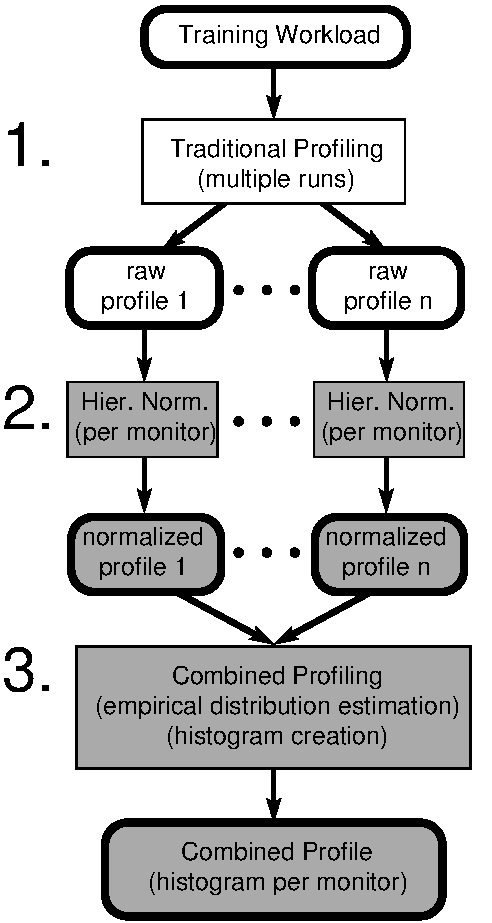
\includegraphics[width=2in]{Figures/cp-overview}
%  \caption{Three phases of combined profiling: 1) profile each input, 2) normalize each profile, and 3) combine the profiles into %a distribution model.}
%  \label{fig:cp-overview}
%\end{figure}

\CP\ and \HN\ have been presented in previous 
work~\cite{BerubeICPE11,BerubeISPASS12}. % However, this presentation
%clarifies and expands on previous versions, particularly the
%description of \CP's histograms in \refSection{cp:empirical} and the
%discussion of queries in \refSection{cp:queries}.
However, a clearer and expanded version, based on previous versions, can
be found in ~\cite{BerubePhD}, particularly the
description of \CP's histograms and the discussion of queries

%\refSection{cp:design} discusses the design of \CP, and the details of
%the technique are presented in \refSection{cp:empirical}.  \CP\ is
%widely applicable; \refSection{cp:extend} briefly discusses the use
%of \CP\ with additional forms of profiling.

%\begin{figure*}[h!]  % fullpage figures should always be at the top
%  \centering
%
%  \makebox[\linewidth][t]{
%  %  \centering  % centering does not seem to be working inside the box...
%
%    \subfigure[A control flow graph.  Edges are labeled with the raw
%      frequencies for \{P1, P2, P3\}.  The probabilities that the left
%      branch is taken from nodes $A$ and $B$ are listed in the
%      adjacent boxes.]{
%      \label{fig:motivate:cfg}
%      \begin{minipage}[b]{0.48\textwidth}
%        \centering
%        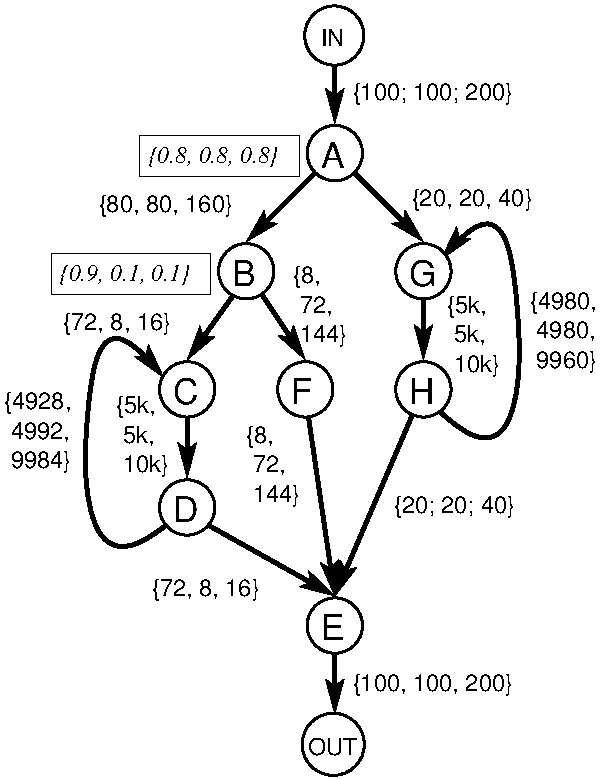
\includegraphics[width=\textwidth]{Figures/motivate}
%      \end{minipage}
%    } % end subfigure a 
%    \subfigure[The edge-dominator tree for \refFigure{fig:motivate:cfg}.]{
%      \label{fig:motivate:domtree}
%      \begin{minipage}[b]{0.48\textwidth}
%        \centering
%        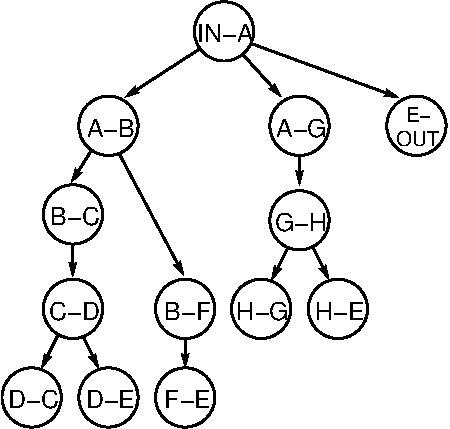
\includegraphics[width=\textwidth]{Figures/domtree}
%        \vspace{0.25in}
%      \end{minipage}
%    } % end subfigure b
%  }\\ % end makebox
%
%%    \hspace{0.15in} % Space between the figures; push table to right
%%                    % margin (compensates for lack of centering...)
%    
%    \subfigure[Profiles P1, P2 and P3 show raw edge frequency counts.
%      P1', P2', and P3' are hierarchically-normalized profiles suitable
%      for combined profiling.]{
%      \centering
%      \label{fig:motivate:eprof} 
%      \begin{minipage}[b]{\linewidth}
%        \centering
%%        \scriptsize
%        % The table will *JUST* fit in a column if it is enclosed by
%        % \begin{small}.  This would allow a 1-col stacked figure.
%        

% the \hspace is a trick to reduce the space taken by the empty column
% between section of the table (vs just leaving it empty)
\begin{tabular}{r@{$\rightarrow$}lr@{$\rightarrow$}lr@{\hspace{0.01in}}rrrr@{\hspace{0.01in}}rrr}

\multicolumn{2}{c}{} & \multicolumn{2}{c}{} 
  & & \multicolumn{3}{c}{\bf Raw}
  & & \multicolumn{3}{c}{\bf Normalized} \\  \cline{6-8} \cline{10-12}
\multicolumn{2}{c}{\bf Edge} \T & \multicolumn{2}{c}{\bf Dom}
  & & {\bf P1}  & {\bf P2}  & {\bf P3}
  & & {\bf P1'} & {\bf P2'} & {\bf P3'} \\ \hline

IN&A \T & \multicolumn{2}{c}{} 
             &&   100   & 100   & 200     &&   1.0  & 1.0 & 1.0 \\
A&B   & IN&A &&   80    & 80    & 160     &&   0.8  & 0.8 & 0.8 \\
A&G   & IN&A &&   20    & 20    & 40      &&   0.2  & 0.2 & 0.2 \\
G&H   & A&G  &&   5,000 & 5,000 & 10,000  &&   250  & 250 & 250 \\
H&G   & G&H  &&   4,980 & 4,980 & 9,960   &&   249  & 249 & 249 \\
H&E   & G&H  &&   20    & 20    & 40      &&   4.0e-3  & 4.0e-3 & 4.0e-3 \\
B&C   & A&B  &&   72    & 8     & 16      &&   0.9  & 0.1 & 0.1 \\
C&D   & B&C  &&   5,000 & 5,000 & 10,000  &&   69.4 & 625 & 625 \\
D&C   & C&D  &&   4,928 & 4,992 & 9,984   &&   1.0  & 1.0 & 1.0 \\
D&E   & C&D  &&   72    & 8     & 16      &&   1.4e-2  & 1.6e-3 & 1.6e-3 \\
B&F   & A&B  &&   8     & 72    & 144     &&   0.1  & 0.9 & 0.9 \\
F&E   & B&F  &&   8     & 72    & 144     &&   1.0  & 1.0 & 1.0 \\
E&OUT & IN&A &&   100   & 100   & 200     &&   1.0  & 1.0 & 1.0 \\ \hline

\end{tabular}
\\
%        ~ % without this space on a new line, the minipage has no
%          % actual line of text, and the alignment of the subfigures
%          % gets all screwed up.
%%        \vspace{0.25in}  % push the table up from the bottom of the figure
%      \end{minipage}
%    } % end subfigure c
%
%  \caption{The \CFG\ and  edge-dominator tree of a procedure, with three possible edge profiles}
%  \label{fig:motivate}
%\end{figure*}


\CP\ ~\cite{BerubePhD} provides a data representation for profile information, but does
not specify the semantics of the information stored in the combined
profile.  Raw profiles cannot be combined naively. %To illustrate this
%point, \refFigure{fig:motivate:cfg} presents a \CFG\, and the table in
%\refFigure{fig:motivate:eprof} provides the edge frequencies observed
%for three profiles: P1, P2, and P3. The numbers within the rectangles
%are the probabilities for edges A$\rightarrow$B and
%B$\rightarrow$C. First note that averaging values across profiles is
%misleading because it can easily characterize behavior in a way that
%does not correspond to any individual profile; The average branch
%probability at B is 0.37, hiding its strongly biased behavior.  In all
%three profiles, the probability of entering the G-H loop from A is
%0.2.  The loop trip counts for P1 and P2 are identical, but the
%probability of entering the C$\rightarrow$D loop from B is 0.9 in P1
%and 0.1 in P2.  P3 is identical to P2, except that all edge counts are
%doubled.  Therefore, P2 and P3 are essentially the same profile; if
%they were combined, the resulting profile should not show any
%variation in program behavior.  However, if the two raw frequencies
%for an edge such as G$\rightarrow$H were combined into a histogram,
%the values 5,000 and 10,000 would not suggest this consistent
%behavior.

%On the other hand, the raw frequencies for edge C$\rightarrow$D in
%P1 and P2 are both 5,000, but P1 enters the loop much more frequently
%than P2 due to the 0.9 vs 0.1 branch probability at B.  Therefore,
%the average trip count of the loop in P1 is much lower (69.4) than in
%P2 (625). In this case, histogramming the raw frequencies
%suggests consistent behavior for the loop, which is misleading.

\subsection{Hierarchical Normalization}
\label{cp:hn}

There is a problem when pairs of measurements are taken under different
conditions.  Thus, when
combining these measurements, all values recorded for a monitor must
be normalized relative to a common fixed reference.  {\em Hierarchical
  normalization} (\HN) ~\cite{BerubePhD} is a profile semantic designed for use with
\CP\ that achieves this goal by decomposing a \CFG\ into a hierarchy
of dominating regions.
%The results of using \HN\ for the profiles in
%\refFigure{fig:motivate:eprof} are shown in the right portion of the
%table.  As desired, P2 and P3 are identical, and the differences in
%loop trip count between P1 and P2 are identified.

%\HN\ is presented for vertex profiling.
\HN\ is presented for edge profiling.  Vertex profiles are treated
identically, but use the domination relationships between vertexes
instead of edges.  Domination is usually defined in terms of vertexes.
In order to use an existing implementation of a vertex dominator-tree
algorithm with edge profiles, use the line graph of the \CFG\ instead of
the \CFG\ itself.  The line graph contains one vertex for each edge in
the \CFG, and edges in the line graph correspond to adjacencies
between the edges of the \CFG.
%This technique may be similarly applied to a call-graph.

%Decomposing a \CFG\ into a hierarchy of dominating regions to enable
%\HN\ is achieved by constructing its dominator tree. Each edge in the
%\CFG\ is represented by a node in the dominator tree.  Denote the
%immediate proper dominator of \CFG\ edge $e$ by $dom(e)$.  Each non-leaf
%node $n(e)$ in the dominator tree is the head of a region $G_e$, which,
%by construction, encompasses any regions entered through descendants of
%$e$.  To prepare a raw profile for combination with other profiles,
%the frequency $f_e$ of each non-root node $n(e)$ is normalized against
%the frequency of its immediate proper dominator, $f_{dom(e)}$.
%The ratio of these two frequencies is invariant when a branch
%probability or loop iteration count is (dynamically) constant.
%This process also prevents variable behavior in an outer loop from masking
%consistent behaviors within the loop.  Normalization proceeds in a
%bottom-up traversal of the dominator tree, so that the head of a
%region is normalized to its immediate dominator only after all of its
%descendents have been normalized.  The root of the dominator tree,
%\ie, the edge representing entry into the procedure, is assigned a
%``normalized'' value of 1.

%In order to understand the capabilities and limitations of a
%statistical model incorporating \HN, and to use it correctly, the
%model must be precisely defined.  Therefore, let $\fancy{F}_e$ and
%$\fancy{F}_{dom(e)}$ be random variables for the raw frequencies of
%$e$ and $dom(e)$, respectively.  Define a new random variable $Y_e =
%\frac{\fancy{F}_e}{\fancy{F}_{dom(e)}}$, which is the frequency of
%edge $e$ with respect to its dominator.  The raw profile from run 1 of
%the program records $f_{dom(e)}^1$ and $f_e^1$, the observed
%frequencies of the two nodes over that run.  One sample of $Y_e$,
%$y_e^1 = \frac{f_e^1}{f_{dom(e)}^1}$ is calculated as the
%hierarchically normalized value for $e$.  Over $k$ runs, $k$ samples
%$y_e^1, y_e^2, ..., y_e^k$ are added to the histogram of $R_e$.  Thus,
%the histogram of monitor $R_e$ is an approximation for the true
%probability density $R_e^*$ ~\cite{BerubePhD}:

%$$ \P(R_e \le \theta) \approx \P(R_e^* \le \theta) = \P \left(Y \le \theta\right) = \P \left(\frac{\fancy{F}_e}{\fancy{F}_{dom(e)}} \le \theta \right)$$

%$$ \P(\alpha \le R_e \le \beta) \approx \P(\alpha \le R_e^* \le \beta) = \P \left(\alpha \le Y \le \beta\right) = \P \left( \alpha \le \frac{\fancy{F}_e}{\fancy{F}_{dom(e)}} \le \beta \right)$$

%$ \int_0^{\theta} R_e \approx \int_0^{\theta} R_e^* = \P \left(Y \le \theta\right) = \P \left(\frac{\fancy{F}_e}{\fancy{F}_{dom(e)}} \le \theta \right)$$




\subsection{Denormalization}
\label{cp:denorm}

The properties of a monitor $R_a$ can only be directly compared to
those of a monitor $R_b$ when $dom(a) = dom(b)$.  However, more
generalized reasoning about $R_a$ may be needed when considering code
transformations.  Similarly, when code is moved by a transformation,
its profile information must be correctly updated. {\it
  Denormalization} reverses the effects of hierarchical normalization
to lift monitors out of nested domination regions by marginalizing-out
the distribution of the dominators above which they are lifted.
Denormalization is a heuristic method rather than an exact statistical
inference because it assumes statistical independence between monitors.
%inference because it assumes statistical\footnote{$R_i$,$R_j$ are
%  independent iff $ \forall i,j:\P(R_i=i,R_j=j) = \P(R_i=i)\P(R_j=j)$.
%  Control-flow equivalence implies independence. Independence does not
%  hold in most other cases.}  independence between monitors.

%Consider first the hierarchically-normalized raw profiles in
%\refFigure{fig:motivate}.  Intuitively, the expected execution count
%of node $F$ for a single execution through the graph is calculated:
%\begin{eqnarray*}
%\mathrm{BP}_l(A) &=& \left(\frac{f_{A\leftarrow B}}{f_{A\leftarrow B} + f_{A\leftarrow G}}\right) \\
%\mathrm{BP}_r(B) &=& \left(\frac{f_{B\leftarrow F}}{f_{B\leftarrow C} + f_{B\leftarrow F}}\right) \\
%\E[f_F] &=& \E[R_{IN\leftarrow A} \times \mathrm{BP}_l(A) \times \mathrm{BP}_r(B)]\\
%\mathrm{P1}:\E[f_F] &=& 1.0 \times 0.80 \times 0.90 = 0.72 \\
%\mathrm{P2, P3}:\E[f_F] &=& 1.0 \times 0.80 \times 0.10 = 0.08
%\end{eqnarray*}
%where $\mathrm{BP}_d(n)$ is the probability of a branch going in
%direction $d$ (either (l)eft or (r)ight) from node $n$.  However, even
%a single raw profile is a statistical model. Thus, the calculation
%above assumes that the edge frequencies are independent.
  
%With the same assumption, the same approach can be used with a \CP.
%Thus, for the \CP\ built from P1, P2 and P3:
%$$ \E[f_F] = 1.0 \times 0.8 \times \left(\frac{0.9+0.1+0.1}{3}\right) = 0.29 $$ 
%which is the average of the expected frequencies.

%The mean is a special case of marginalization; independence allows the
%joint distribution to be broken into the product of individual
%distributions, where the expectation associates over the product,
%simplifying the calculation to the product of means seen above.  Thus,
%to recover an ``absolute'' expected execution count from an
%\HN\ \CProf, multiply the means of each monitor up the dominator tree
%to the procedure entry.  Then, multiply by the expected invocation
%frequency of the procedure (possibly using this technique over a
%\CG\ \CProf).  Denormalization is this process of multiplying monitors
%along a path in the dominator tree.  The mean is a special case of
%denormalization because it does not require the distribution of
%monitor values.  The general denormalization technique is formally
%presented in the remainder of this section.

%Let $R_a$ and $R_b$ be monitors from the same \CFG.  Let
%$\mathit{dom}^i(R_a)$ be the $i^{th}$ most-immediate proper dominator
%of $R_a$.  The least-common dominator of $R_a$ and $R_b$ is $R_d =
%\mathit{dom}^j(R_a) = \mathit{dom}^k(R_b)$, where there is no monitor
%$R_n$ such that $R_d$ properly dominates $R_n$, and $R_n$ dominates
%both $R_a$ and $R_b$.  Denormalizing $R_a$ from the region dominated
%by $\mathit{dom}(R_a)$ to the region dominated by $R_d$ is achieved by
%walking up the dominator tree.  Let $\widehat{R_n^{-i}}$ be the
%denormalized distribution when $R_n$ is lifted above $dom^i(n)$.
%$\widehat{R_n^{-1}}$ is created by multiplying together the histograms
%$H_n$ and $H_{dom(n)}$. Denormalization can be applied to $R_a$ and
%$R_b$ recursively to produce the desired $\widehat{R_a^{-j}}$ and
%$\widehat{R_b^{-k}}$, which can be compared ~\cite{BerubePhD}.

%The computation of $\widehat{R_n^{-i}}$ takes $O(ib^2)$ time, assuming
%that all histograms use $b$ bins.  The number of bins is chosen by the
%user. There is a tradeoff between accuracy and precision on one hand
%and memory space and computation time on the other.

%\begin{figure}
%  \centering
%  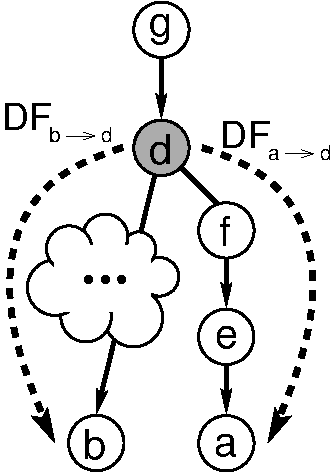
\includegraphics[width=0.3\linewidth]{Figures/denormalize}
%  \caption{Denormalization of $R_a$ and $R_b$ with respect to their
%    least-common dominator $R_d$.  Dashed lines show the path over
%    which the marginalized histograms are computed.}
%  \label{fig:denormalize}
%\end{figure}

%\refFigure{fig:denormalize} shows a dominator tree containing the
%nodes $a$ and $b$ and their least common dominator $d$, which is
%shaded.  The dashed lines illustrate the paths followed, in the
%dominator tree, to compute the denormalization. Nodes $f$ and $e$ are
%in the path from $d$ to $a$ and there might be other nodes in the path
%from $d$ to $b$.  Thus, $R_d = \mathit{dom}^3(R_a)$, and the histogram
%for $\widehat{R_a^{-3}}$ is calculated:
%$$ \widehat{H_a^{-3}} = H_a \times H_e \times H_f \times H_d $$


\subsection{Queries}
\label{cp:queries}

In an AOT compiler, profiles are used to predict program behavior.
Thus, raw profiles are statistical models that use a single sample to
answer exactly one question: {\em ``What is the expected frequency of
  X?''}  where X is an edge or path in a \CFG\ or a Call Graph (\CG).
A \CP\ is a much richer statistical model that can answer a wide range
of queries about the measured program behavior.  The implementation of
\CP\ used in this work provides the following statistical queries as
methods of a monitor's histogram:
\begin{description}

\item[$H.\mathrm{min}, H.\mathrm{max}$]: 
%  The maximum and non-zero
%  minimum monitor value observed, as in ~\cite{BerubePhD}.

\item[$H.\mathrm{mean}(\mathit{incl0s})$]: 
%  The true weighted average of
%  observed monitor values.  If {\it incl0s} is true, count raw
%  profiles where the monitor did not execute as 0-valued observations,
%  as in ~\cite{BerubePhD}.

\item[$H.\mathrm{stdev}(\mathit{incl0s})$]: 
%  The true weighted standard
%  deviation of observed monitor values.  If {\it incl0s} is true,
%  count raw profiles where the monitor did not execute as 0-valued
%  observations, as in ~\cite{BerubePhD}.

\item[$H.\mathrm{estProbLessThan}(v)$]: 
%  Estimates the value of the
%  monitor's CDF at $v$, \ie, $\P(R \le v)$.  The estimation is based
%  on the assumed uniform distribution of bins.

\item[$H.\mathrm{quantile(q)}$]: 
%  For $0 \le q \le 1$, estimates the
%  (minimum) value $v$ at the point where the monitor's CDF equals $q$,
%  \ie, $v$ when $\P(R \le v) = q$.  The estimation is based on the
%  assumed uniform distribution of bins.

\item[$H.\mathrm{applyOnRange}(F(w,v),\mathit{vmin},\mathit{vmax})$]: 
%  Computes the sum of applying the function $F(w,v)$ to the impulses
%  of the histogram in the range $[\mathit{vmin}, \mathit{vmax}]$, as
%  with the multiplication of histograms in ~\cite{BerubePhD}.
%  For bins that partially overlap the range, the impulse's weight is
%  proportional to the overlap of the bin with the range, and the
%  impulse's value is the midpoint of the overlapping range.

\item[$H.\mathrm{applyOnQuantile}(F(w,v),\mathit{qmin},\mathit{qmax})$]: 
%  Like applyOnRange, but the range is set using the values associated
%  with the quantile points {\it qmin} and {\it qmax}.

\item[$H.\mathrm{coverage}$]: 
%  The probability of the monitor executing
%  in a run of the program, computed as $\frac{H.W}{H.\mathit{TW}}$.

\item[$H.\mathrm{span}$]: 
%  The ratio between the range of the histogram
%  and its maximum value, computed as $\frac{H.\mathrm{max} -
%    H.\mathrm{min}}{H.\mathrm{max}}$.

\end{description}


%The mean value of a monitor is analogous to the value provided by a
%single raw profile, and provides the desired substitutability of a
%\CProf\ for a raw profile in existing \FDO\ transformations.
%
%\REM{ along with the standard deviation and minimum and maximum
%  values.  Furthermore, \CP\ can estimate from a monitor's Cumulative
%  Distribution Function (CDF) the probability that the monitor is
%  within a (possibly half-bounded) range.  Conversely, the inverse CDF
%  provides estimates of the thresholds corresponding to a given
%  quantity of probability mass.  For example, the inverse CDF
%  facilitates estimating the median value of a monitor.
%}
%
%The additional statistical information provided by a \CProf\ allows an
%\FDO\ heuristic to quantify the expected trade-offs between various
%workload-performance measurements, such as between the impact on the
%5\%-quantile (nearly worst-case) or the average impact on the
%5\%--95\%-quantile range (omitting potential outliers).  In some
%transformations, the order in which candidates are considered is
%important~\cite{ChakrabartiCGO06}.  \CP\ allows a sorting function to
%use, for example, both the mean and the standard deviation of the
%candidates in order to prioritize low-variance opportunities.
%Behavior variation should not, by itself, inhibit
%optimization. Rather, 
\CP\ enables the accurate assessment of the
potential performance impact of transformations informed by
variable-behavior monitors in a variety of ways, and with adjustable
confidence in the result. Concrete examples of this kind of analysis
are provided by the implementation of an \FDO\ inliner using
\CP\ described in \cite{BerubePhD}.


%\subsection{Extensions and Alternative Usage}
\subsection{Alternative Usage}
\label{cp:extend}

The empirical-distribution methodology of \CP\ is orthogonal to the
techniques used to collect raw profiles.  \CP\ is applicable whenever
multiple profile instances are collected, including intra-run
phase-based profiles, profiles collected from hardware
performance-counter, and sampled profiles.  The main issue when
combining profiles is how normalization should be done in order to
preserve program-behavior characteristics.

%\subsubsection{\CFG\ Paths}
%
%\begin{figure}
%  \centering
%  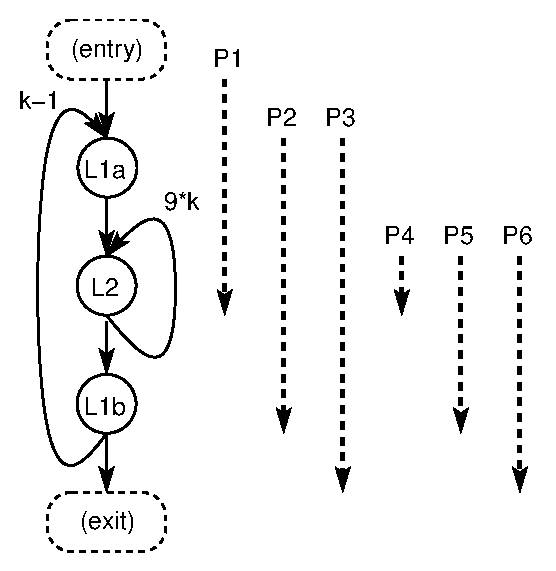
\includegraphics[width=0.50\linewidth]{Figures/pathnorm}
%  \caption{Some sub-paths through a nested loop. The outer loop
%    $L_1$ iterates a total of $k$ times; the inner loop $L_2$ iterates 10
%    times per iteration of $L_1$.}
%  \label{fig:pathnorm}
%\end{figure}
%
%An algorithm that collects path profiling in a program that contains
%loops must break cycles.  The most commonly used technique to break
%such cycles is due to Ball and Larus~\cite{BallLarusMICRO96}. Given a
%simple loop, the main idea is to replace the back edge with a set of
%sub-paths that include (a) a path from a point outside the loop to the
%end of the first iteration, (b) a path from the loop entry point to a
%point outside the loop, and (c) a path from the entry point to the
%exit point in the loop.
% \refFigure{fig:pathnorm} illustrates some of
%the paths inserted to replace the two back edges in a double-nested
%loop.
%
%Hierarchical normalization must be adapted to work with paths because
%there are no dominance relationships between paths. Consider two runs
%of a double-nested loop, where the outer
%loop $L_1$ iterates a total of $k=10,000$ times in the first run, and
%$k=100$ times in the second run.  In both cases the inner loop $L_2$
%iterates 10 times per iteration of $L_1$.  A combined profile should
%identify the path of execution within $L_1$ as consistent across runs,
%but should indicate that the frequency of the paths into and out of
%$L_1$ vary significantly from run to run. The solution is to normalize
%path frequencies with respect to the frequency of the vertex that
%starts the path.  For instance, P4 should be normalized to the
%frequency of $L_2$ to factor out $k$ and preserve the constant nature
%of the inner loop.


%\subsubsection{Program Call-Graphs}

%Combined profiling can easily be extended to call-graphs
%(\CG)\footnote{We do not attempt to extend \CP\ to inter-procedural
%  paths~\cite{MelskiPhd02}.}.  Profiling a \CG\ gathers information
%about the frequency of inter-procedural calls.  A \CG\ can be
%represented in multiple ways.  For instance, a single edge may
%represent all calls from a procedure \funcname{foo()} to a procedure
%\funcname{bar()}.  Alternatively, there may be a separate edge for
%each call-site in \funcname{foo()} that targets \funcname{bar()}. If
%context-sensitivity is included, there are several alternatives to
%keep track of the execution path that leads to a call from
%\funcname{foo()} to \funcname{bar()}.  A common solution is to keep
%track of the $k$ most recent calls on the stack when the call from
%\funcname{foo()} to \funcname{bar()} occurs~\cite{MightPLDI10}.  This
%sequence of calls is called a {\em call string}.

% \pb{Changed based on our discussion for inlining}
%Unlike a \CFG, a \CG\ is not a well-structured graph.  Consequently,
%the dominator tree is often very wide and shallow, which limits the
%utility of applying \HN\ to the full \CG.  Instead, we propose that
%\CG\ monitors are normalized with respect to the invocation frequency
%of the procedure where the behavior originates. In the case of
%\CG\ profiles that do not use context sensitivity, call frequencies
%are normalized against the caller's frequency.  Likewise, when
%context-sensitivity is used to collect a \CG\ profile, call-string
%frequencies are normalized against the frequency of the caller of the
%first call in the string.  The combined profile then provides a
%conditional distribution describing the expected frequency of
%following a call or call string, given that the start of the call
%string has been reached.


%\subsubsection{Value Profiling}

%A monitor $R$ for value profiling observes the run-time values of a
%variable at a specific program point in order to enable specialization
%transformations~\cite{Calder97}.  Each profiling run produces a
%histogram of the frequency of observed values of the variable.
%However, since a variable could potentially take very many different
%values over a program run, a caching technique is used to estimate the
%frequency of the $n$ most frequent values.  Since a value profile is
%completely local to a single program point, there is no hierarchy over
%which to normalize; normalization simply requires converting the
%frequency for each value $v$, $f(v)$, into a proportion of
%the total number of observations, $\P(v)$ (\ie, the probability of
%observing $v$).  The \CProf\ for value profiling then creates a
%histogram for each frequently-observed $v$ over the $\P(v)$ of each
%run.  Thus, the \CProf\ identifies the frequent values of $R$, and the
%distribution of the likelihood of observing each value.  If the set of
%frequent values is not consistent across runs, less-likely values may
%need to be pruned from the \CProf, or the variable may simply be
%marked as unsuitable for specialization.

%\subsubsection{Profiling Granularity}

%This work assumes that \CP\ will combine input profiles from complete,
%single, program runs.  However, the input profiles can have arbitrary
%granularity.  For instance, \CP\ could combine \CFG\ profiles from
%each separate invocation of a function (a finer temporal granularity).
%Similarly, each thread in a concurrent application could contribute a
%separate raw profile for combination into a multi-threaded \CProf\ for
%a single run (thread-level granularity).  In conjunction with phase
%detection, a \CProf\ could be build to represent behavior variation
%between fine-grained program phases.  Conversely, long-running server
%applications could periodically commit profile information to
%a \CProf\ to model program behavior variation over different times of
%day or even different days of the week.


%\REM{
%\section{old stuff}
%Other stuff that is obvious or interesting or has come up in the
%course of research and has been put aside as beyond the scope of this
%work:
%\begin{itemize}
%\item Keep profiles across code changes?
%\item Finer-grained profiling (candidacy: scope)
%\item Value profiling: histograms-of-histograms
%\item \todo{CG profiling, all variations: expand on ISPASS'11}
%\item Inter-procedural path profiling
%\end{itemize}
%}


\section{Function Inlining}
	\label{sec:inlining}
	
Function inlining, or simply inlining, is a classic code
transformation that can significantly increase the performance of many
programs.  A compiler pass that decides which calls to inline, and in
which order, is referred to as an inliner.  The basic idea of inlining
is straightforward: rather than making a function call, replace the
call in the originating function with a copy of the body of the
to-be-called function.  Nonetheless, many inliner designs are
possible; \cite{BerubePhD} describes the existing inliner
in \llvm, and also the alternative
approach used by a new feedback-directed inliner (\FDI) that uses \CP.
All inlining discussed in this paper is implemented in the
open-source \llvm\ compiler~\cite{LattnerAdveCGO04}.

Some terminology is required to identify the various functions and
calls involved in the inlining process.  The function making a call is
referred to as the {\it caller}, while the called function is the {\it
callee}.  The representation of a call in a compiler's {\it internal
representation} (IR) is a {\it call site}; in \llvm, a call site is an
instruction that indicates both the caller and the callee.  Thus,
inlining replaces a call site by a copy of that call site's callee.
When a call is inlined, the callee may contain call sites, which are
copied into the caller to produce new call sites.  The call site where
inlining occurs is called the {\it source} call site.  A call site in
the callee that is copied during inlining is called an {\it original}
call site, and the new copy of the original call site inside the
caller is called the {\it target} call site.

\subsection{Barriers to Inlining}

Not every call site can be inlined.  Indirect calls use a pointer
variable to identify the location of the called code, and arise from
function pointers and dynamically-polymorphic call dispatching.  These
calls cannot be inlined, because the callee is unknown at compiler
time.  External calls into code not currently available in the
compiler, such as calls into different modules or to statically-linked
library functions cannot be inlined before link-time because the
source representation of the callee is not available in the compiler.
Calls to dynamically-linked libraries can never be inlined by
definition. Moreover, if a callee uses a \name{setjump} instruction,
it cannot be inlined. A \name{setjump} can redirect program control
flow {\it anywhere}, including the middle of different function,
without using the call/return mechanisms.  Inlining the \name{setjump}
could cause any manual stack management at the target of the jump to be
incorrect; the inlined version would not be functionally equivalent to
the original.

\subsection{Benefits of Inlining}

Inlining a call has a small direct benefit.  Removing the call reduces
the number of executed instructions.  The {\tt call} instruction in
the caller is unnecessary, as is the {\tt return} instruction in the
callee.  Furthermore, any parameters passed to the callee and any
values returned no longer need to be pushed onto the
stack\footnote{Some calling conventions allow values to pass between
  the caller and callee in registers.}.

\begin{figure}
  \centering
  
  \begin{minipage}[t]{\linewidth}
    \subfigure[Original code fragment] {
      \begin{minipage}[b]{0.45\textwidth}
        \centering
        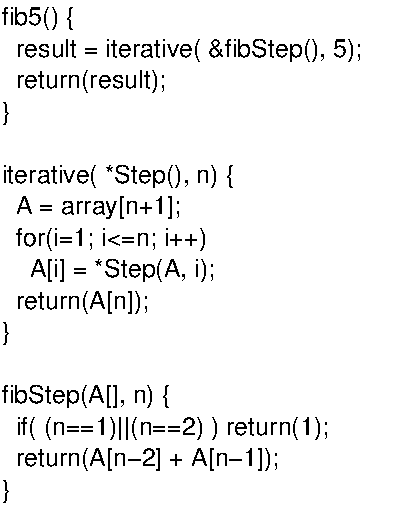
\includegraphics[height=12em]{Figures/fibiter-1}
      \end{minipage}
      \label{fibiter:orig}
    }
    \subfigure[after inlining \iname{iterative}] {
      \begin{minipage}[b]{0.45\textwidth}
        \centering
        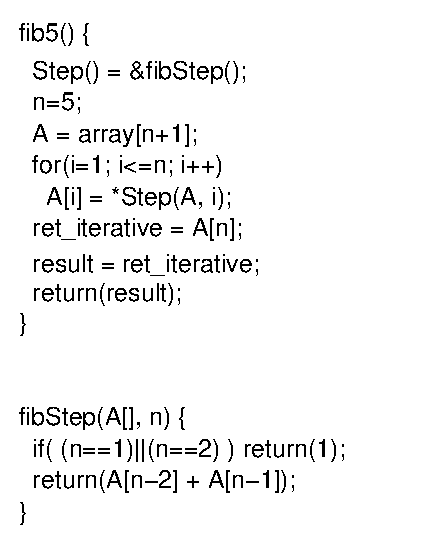
\includegraphics[height=12em]{Figures/fibiter-2}
      \end{minipage}
      \label{fibiter:iterative}
    }
    \vspace{1em}
    \hrule
    \vspace{1em}
  \end{minipage}
  \begin{minipage}[t]{\linewidth}
    \centering
    \subfigure[after constant and copy propagation] {
      \begin{minipage}[b]{0.25\linewidth}
        \centering
        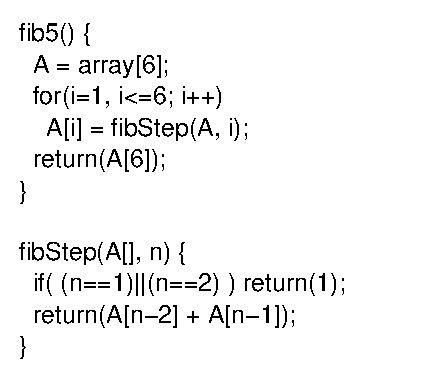
\includegraphics[height=8.8em]{Figures/fibiter-3}
      \end{minipage}
      \label{fibiter:prop}
    }
    \hspace{0.07\linewidth}
    \subfigure[after inlining \iname{fibStep} and simplification] {
      \begin{minipage}[b]{0.25\linewidth}
        \centering
        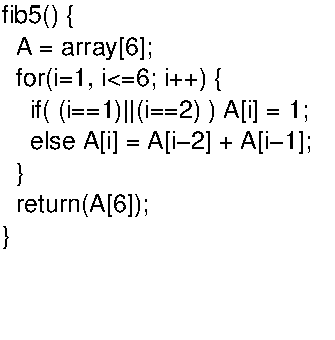
\includegraphics[height=8.8em]{Figures/fibiter-4}
      \end{minipage}
      \label{fibiter:fibstep}
    }
    \hspace{0.07\linewidth}
    \subfigure[after loop unrolling and scalar promotion] {
      \begin{minipage}[b]{0.24\linewidth}
        \centering
        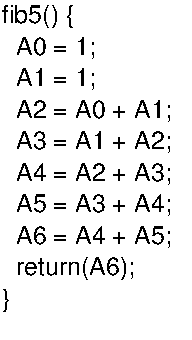
\includegraphics[height=8.8em]{Figures/fibiter-5}
      \end{minipage}
      \label{fibiter:final}
    }
  \end{minipage}
  \caption{A sequence of transformations on a code fragment that
    computes Fibonacci numbers, illustrating the code-simplification
    opportunities enabled by inlining ~\cite{BerubePhD}}
  \label{fig:fibiter}
\end{figure}

However, the greatest potential benefit of inlining comes from
additional code simplification it may enable by bringing the callee's
code into the caller's scope. \refFigure{fig:fibiter} presents a
running example demonstrating the transformations that become possible
due to inlining.  Many code analysis algorithms work within the scope
of a single function; inter-procedural analysis is usually
fundamentally more difficult, and always more computationally
expensive than intra-procedural analysis, because of the increased
scope.  A function call inhibits the precision of analyses and is a
barrier to code motion because the caller sees the callee as a ``black
box'' with unknown effect.

%As discussed above, inlining a call directly reduces the number of
%executed instructions. Both the \llvm\ and \FDI\ inliners estimate
%these savings as 10 instructions for the call, plus one instruction
%per parameter.  The analyses used to determine the additional benefits
%of inlining a call site do so by estimating the number of instructions
%in the inlined code that will be eliminated after inlining.
%Therefore, the estimate is for the static number of instructions, or
%code size, rather than the dynamic number of instructions executed at
%run time.  Code size reduction is estimated for constant parameters
%and stack-allocated arrays passed by pointer, on a per-parameter
%basis.

%The same straight-forward analysis is used by both inliners to
%estimate the impact of each parameter.  When analyzing a parameter,
%the \llvm\ inliner counts the number of instructions eliminated, and
%adds bonus ``instruction-equivalent'' savings for beneficial
%situations that do not directly eliminate instructions.  Instead of
%adding bonuses to a grand total during the analysis, the \FDI\ inliner
%maintains separate counts for each indirectly-beneficial situation.

%The analysis for stack-allocated arrays passed by pointer is
%essentially the same as the constant-parameter analysis.  The base
%address of the array becomes a constant that can be propagated, while
%the array data is known to reside on the stack.  This additional
%information enables transformations that treat the array locations as
%scalar values\footnote{\eg, scalar promotion, loop-invariant code
%  motion}.  
  For example, after loop unrolling and scalar promotion,
the code in \refFigure{fibiter:fibstep} is transformed into the code in
\refFigure{fibiter:final}.  Constant propagation in that final version of
the code allows the compiler to replace the entire initial computation
of \iname{fib5} by the constant value 13.  However, the analysis does
not consider the potential impact of such transformations, but only
count instructions directly eliminated because the array's base
address is a constant.

The impact of a constant parameter is determined for each formal
parameter of each function in advance, by assuming that it takes a
constant, but unknown, value.  \llvm's IR uses a {\it single static
  assignment} (SSA) representation, where each {\tt value} produced is
defined exactly once.  Data flow is represented by directly linking
each {\tt value}\footnote{Formal parameters and IR instructions are
  both {\tt values}.}  to the instructions that use it.  
%Each IR
%instruction $u$ using parameter $p$ is examined, assuming that $p$
%takes a constant value.  If $u$ is neither a branch nor a call
%instruction, then if all of $u$'s inputs are constants, it can be
%eliminated by constant folding.  When $p$ is the only non-constant
%input to $u$, $u$ is counted as an eliminated instruction, and the
%analysis continues recursively to the uses of $u$.

When $u$ is an indirect call for which the callee becomes constant,
the call is resolved to a direct call.  \llvm\ awards a large bonus
for this conversion; \FDI\ counts the conversion separately from other
eliminated instructions.

%If $u$ is a branch or switch instruction who's test condition becomes
%constant, the control-flow outcome of the branch is restricted to a
%single possibility.  However, since the value of $p$ is unknown, the
%actual outcome of the branch is also unknown.  Each of the $n$ possible
%outcomes are considered equally likely.  The average size of the
%blocks corresponding to the possible outcomes, $\overline{s}$, is
%determined.  Only one outcome is possible, thus $\overline{s}(n-1)$
%instructions are expected to be eliminated. 
\llvm\ does not include
the (now-unconditional) branch instruction in the count of eliminated
instructions. \FDI\ counts eliminated branch instructions separately
from other eliminated instructions.  The analysis does not continue to
subsequent successor blocks.

In the evaluation of the inlining benefit of a particular call site,
the benefit pre-computed for the callee's formal parameters is
retrieved, as appropriate, for each actual parameter that is a constant
or a pointer to a stack-allocated array.  The impact of each parameter
is accumulated to estimate the total code-size reduction enabled by
inlining the call site.  The \llvm\ inliner simply adds these values
together.  \FDI\ adds the counts for each category it measures and
then computes a weighted sum of those values, as explained in detail in
\cite{BerubePhD}.

\subsection{Costs of Inlining}

Inlining non-profitable call sites can indirectly produce negative
effects.  The increased scope provided for analysis by inlining also
increases the costs of these analyses.  Most algorithms used by
compilers have super-linear time complexity.  Extremely large
procedures may take excessively long to analyse; some compilers will
abort an analysis that takes too long.  Furthermore, a program must be
loaded into memory from disk before it can be executed.  A larger
executable file size increases a program's start-up time.  Finally,
developers eschew unnecessarily large program binaries because of the
costs associated with the storage and transmission of large files for
both the developer and their clients. Therefore, inlining that does
not improve performance should be avoided.

\subsection{Inlining-Invariant Program Characteristics}

While inlining a call causes a large change in the caller's code, it
has a minimal direct impact of the use of memory system resources at
run time.  Ignoring the subsequent simplifications the inlining
enables, inlining proper has no appreciable impact on register use, or
data or instruction cache efficiency.  Regardless of inlining, the
same dynamic sequence of instructions must process the same data in
the same order to produce the same deterministic program result.

Inlining should have negligible impact register spills.  The
additional variables introduced into the caller by inlining place
additional demands on the register allocator, and may increase the
number of register spills introduced into the caller.  However,
without inlining, the calling convention requires the caller to
save any live registers before making a call, or for the callee to
save any registers before it uses them; in both cases, these
registers must be restored before resuming execution in the caller.
Thus, inlining merely shifts the responsibility for register
management from the calling convention to the register allocator.

Similarly, inlining does not change the data memory accesses of a
program.  Whether in the caller or the callee, the same loads and
stores, in the same order, are required for correct computation.
Subsequent transformations may reorder independent memory accesses to
better hide cache latency, or eliminate unnecessary accesses
altogether, but this is not a direct consequence of inlining.  Thus,
data cache accesses do not change with inlining, and nor does the
cache miss rate.  

%Likewise, the same instruction sequence, minus the call and return
%instructions, is executed regardless of inlining.  Given a
%fully-associative cache with sufficiently small lines, instruction
%cache activity will be identical in either case.  However, caches are
%set associative, and have lines that hold many instructions.
%Therefore, instruction cache efficiency can change if
%frequently-executed instructions are more often adjacent to
%infrequently-executed instructions in the inlined code, and this
%adjacency is contained within a cache line.  A block placement
%algorithm linearizes the basic blocks in a function in order to place
%it in the linear memory address space.  Block placement attempts to
%follow a block in the linear sequence by its most likely successor.
%Given the same block placement algorithm for both the inlined and
%non-inlined versions of the code, there is no reason to believe that
%inlining will cause the algorithm to be less effective at separating
%hot and cold code.  Furthermore, even if hot code more frequently
%shares a cache line with cold code, this situation will only cause a
%small increase in the number of cold misses in the instruction cache.  Unless the
%hot code no longer fits within the instruction cache, the steady-state
%miss rate will not change.  On the other hand, the potentially reduced
%total code size in the case of inlining can only increase the
%effectiveness of instruction caching.


\section{\CP-Driven Feedback-Directed Inliner for \llvm}
	\label{sec:fdi}
	
The feedback-directed inlining (\FDI) ~\cite{BerubePhD} evaluated in this work is
fundamentally different than the existing static inliner in \llvm.
The static inliner inlines small calls to remove call overhead with
minimal increases in code size.  \FDI\ attempts to minimize the
dynamic number of instructions executed by the program by inlining the
most frequent calls.  While the static inliner considers call sites on
a function-by-function basis, \FDI\ considers the set of inlining
opportunities present at global scope in the current state of the
program.

% Remove the ``then'' keyword from if statements
\SetKwIF{If}{ElseIf}{Else}{if}{}{else if}{else}{endif}
\begin{algorithm}[t!p]
\begin{small}
  \SetKwInOut{Input}{input}\SetKwInOut{Output}{output}

  \Input{Module M: Whole-program IR}
  \Input{File cpFile: Combined profile}

  \KwData{List$<$call site$>$ candidates, ignored}
  \KwData{Map$<$Function $\rightarrow$ List$<$call site$>$ $>$ callers}

  initialize(M, cpFile)\label{wl:init}\;
  budget = computeCodeGrowthBudget()\label{wl:budget}\;
  candidates.sort()\;

  %\tcp{Inline the best candidate until the budget is exhausted or 
  %     there's nothing left to inline}
  \While{budget $> 0$  AND NOT candidates.empty}
  {
    %\tcp{remove best candidate}
    source = candidates.popBest()\label{wl:pop}\;

    %\tcp*{the best candidate should not be inlined!}
    \If{source.score $\le 0$\label{wl:ifscore}}
    {
      {\bf break}\;
    }

    %\tcp{already know that callee cannot be inlined}
    \If{source.callee.cannotInline\label{wl:ifcannot}}
    {
      ignored.add(source)\;
      {\bf continue}\;
    }

    %\tcp{too big for remaining budget; skip it}
    \If{source.expectedCodeGrowth $>$ budget\label{wl:ifbig}}
    {
      ignored.add(source)\;
      {\bf continue}\;
    }
      
    \tcp{Try to inline the candidate...}
    inlineResult = LLVM.inlineIfPossible(source)\label{wl:inline}\;
    \If{inlineResult.failed}
    {
      source.callee.setCannotInline()\;
      ignored.add(source)\;
      {\bf continue}\;
    }
%    {
      \tcp{Inlining succeeded}
      %\tcp{update budget using real code growht}
      budget -= inlineResults.codegrowth\label{wl:cost}\;
      %\tcp{the call site no longer exists}
      callers[source.getCallee].delete(source)\label{wl:delcaller}\;
      %\tcp{recalculate the score for the callers; their callee's size has changed}
      \For{caller $\in$ callers[source.caller]\label{wl:evalcallers}}
      {
        caller.calcScore()\;
      }
      %\tcp{deal with any new call sites created by inlining}
      \For{i $\leftarrow$ 1 \KwTo\ inlineResults.numInlinedCalls\label{wl:newcalls}}
      {
        target = inlineResults.inlinedCall[i]\label{wl:newcand}\;
        original = inlineResults.originalCall[i]\label{wl:orig}\;
        callers[target.getCallee].insert(target)\;

        \eIf{ignored.contains(original) $> 0$\label{wl:invalid}}
        {
          target.histogram = 0\;
          ignored.add(target)\;
        }
        {
          target.histogram = source.histogram $\times$ original.histogram\label{wl:newhist}\;
          target.calcScore()\;
          candidates.insert(target)\;
        } % eIf
      } % For
%    } % eIf
 }

\end{small}
  \caption{\FDI\ worklist}
  \label{alg:fdiworklist}
\end{algorithm}

What \FDI\ does is to set the problem as one of constrained minimization,
the {\it Substitution Problem}. So, for a particular program, a subset of
all invocations, the values of maximum program size, maximum callee size,
etc, find a sequence of substitutions that can minimize the expected
program execution time. And this is done by following the order of the
candidate call sites in the candidates list. The list is ordered by the
score of each candidate.

The assumption is that this is an efficient reduction of the Knapsack
Problem to the Substitution Problem \cite{Arnold00,Scheifler1977}. The
Knapsack Problem is known to be NP-hard \cite{Garey1979}, so it's
intractable. To peform the reduction, we first assume that it is
possible to construct an invocation with any integral execution time
overhead. The second assumption is that it is possible to construct a
procedure of any integral size less than the maximum.

\rr{Hidden text extracted from Scheifler1977}
%We define the maximum procedure size so that all
%substitutions are possible, but we constrain the maxi-
%mum program size increase to k. By construction, the
%execution time saved by any sequence of substitutions
%will be exactly the same as the resultant size increase,
%and so the maximum time savings possible is k. If there
%is a subsequence of S that sums to k, then there is a
%sequence of substitutions that will obtain the maximum
%time savings. Conversely, if there is a sequence that
%obtains the maximum time savings, then there is a
%subsequence of S that sums to k. Hence we can solve
%the Knapsack Problem by solving the Substitution
%Problem. Any tractable solution to the Substitution
%Problem is thus a tractable solution to the Knapsack
%Problem, for we can certainly perform the above con-
%struction in polynomial time.
%
%The reduction we have given depends on the fact
%that the maximum procedure size and maximum pro-
%gram size can be made arbitrarily large. If there are
%absolute bounds on these sizes, it may be possible to
%solve the Substitution Problem in polynomial time.
%However, as long as the bounds are reasonably large,
%the polynomial will be of very high degree, and so the
%problem is still essentially intractable.
%
%In view of the above, it is reasonable to take an
%engineering approach and make certain approxima-
%tions in a manner that will arrive, we hope, at a near-
%optimal solution. To begin, we need some measure of
%size and some measure of the execution time overhead
%for any given invocation. The size change resulting
%from a substitution is easy to compute, but we need a
%method for determining how the overhead of an invo-
%cation changes as other invocations are expanded. We
%make several practical approximations to fulfill these
%needs and then return to the actual problem solution at
%the end of this section)
%
%The algorithm we choose has three distinct phases.
%At each step in the first phase, every substitution that
%will result in a nonpositive basic size change is per-
%formed, independent of the time saved; the process
%repeats until no further substitutions are possible by
%this rule. The basic size change for a substitution is the
%change in the size of the procedure body containing the
%invocation. The reduction in program size possible if
%the called procedure can be removed is n o t counted in
%the basic size change, but it/s counted in determining
%the program size after the substitution. We use the
%basic size change in an attempt to keep procedure sizes
%small. As a heuristic, we would rather substitute a small
%frequently called procedure often than expand one in-
%vocation of a very large procedure within that small
%procedure.
%
%The second phase is the heart of the algorithm. At
%each step, the invocation with the highest ratio of
%expected executions to basic size change, whose expan-
%sion will not violate the procedure size constraint, is
%expanded. Any invocations created by the substitution
%are available at the next step. The order of substitution
%can be computed very cheaply by using this rule, but
%there are no mathematical guarantees that the result
%will be near-optimal. 4 The hope, of course, is that good
%results are obtainable for this specific application and
%that more expensive calculations are not required. Sub-
%stitutions continue according to this rule until the maxi-
%mum program size is just exceeded. We prefer not to
%complicate the rule to avoid violating the size con-
%straint; the maximum is, after all, only approximate,
%and in general the additional increase will be small.
%
%Once the second phase is complete, it still may be
%possible to expand some invocations without increasing
%the total program size. When a nonrecursive procedure
%has exactly one invocation to it remaining in the entire
%program and the procedure is known not to be called by
%any other mechanism, expansion of the invocation also
%allows the procedure to be removed, and little if any
%total size increase is involved. All such expansions that
%do not violate the procedure size constraint are per-
%formed in the third and final phase.

\subsection{Worklist Algorithm}

\refAlgorithm{alg:fdiworklist} presents an outline of the worklist
algorithm used by \FDI.  The algorithm uses several data structures:
\begin{description}

\item[{\it candidates}]: \\
  The worklist is a sorted list of candidates.
  A call site is an inlining candidate if it is a direct call, and if
  the callee does not contain a \name{setjump} nor has any previous
  attempt to inline the callee failed.  Furthermore, the call site
  must have executed at least once during profiling.

\item[{\it ignored}]: \\
  A list of call sites that are not inlining
  candidates.  This list is maintained to enable correct and efficient
  bookkeeping, and to allow any copies of these call sites created by
  inlining their caller to be immediately ignored.

\item[{\it callers}]: \\
  A mapping from functions to the call sites that
  call them.  This map allows for the re-scoring of call sites on the
  event that a call is inlined into their callee.  That inlining will
  change the callee's size, and may change the expected
  simplifications possible if the callee is inlined.

\item[{\it inlineResult}]: \\
  A structure returned by inliner that
  provides summary information regarding the transformation.  In
  particular, it indicates if the attempted inlining failed.
  \FDI\ enhances the default \llvm\ structure with co-indexed lists
  identifying the new call sites created in the caller by inlining,
  and their originating call sites in the callee.  This information is
  required so that profile information can be estimated for the new
  call sites.

\end{description}

At the start of \FDI, the \CProf\ is read in, and the histograms are
associated with the appropriate call sites (\refLine{wl:init}).  Every
call site is inserted into the callers list of their callee.  During
initialization, each call site is evaluated, and added to either the
candidates or ignored list, as appropriate.  When a call site is
rejected for inlining, it is immediately and permanently moved from
the list of candidates to the ignore list.  Transformations such as
constant propagation or alias analysis can resolve the callee of an
indirect call to a single possibility, thereby making it a direct
call.  However, if the call is indirect when the call site is first
discovered by the inliner, it is placed on the ignore list in spite of
the possibility of future inlining resolving the call.  Calls to
libraries and compiler built-in functions are also immediately ignored
because they cannot be inlined.

\subsection{Candidate Scoring}
\label{inlining:scoring}

The \llvm\ inliner makes inlining decisions at each call site by
comparing the expected code growth to a fixed threshold.  \FDI\ takes
a more directly execution-time-oriented approach to inlining and
attempts to achieve the greatest reduction in executed instructions
for the least amount of code growth.  Therefore, \FDI\ breaks the
evaluation of a call site into three components: the expected inlining
benefit, the expected code growth, and execution frequency of the call
site.  Given a call site, \CS, the inlining candidate scoring
function, \ScoreOf{\CS}, combines these three elements so
that \refAlgorithm{alg:fdiworklist} can select the best (highest
score) candidates for inlining first. \CP\ provides a rich
characterization of execution frequency. Making use of that
information is described in detail in \cite{BerubePhD}; for
now, let $\RewardOf{\BenefitOf{\CS}, R_{\CS}}$ represent some function
of the estimated (execution-frequency independent) inlining benefit at
call site \CS\ and $R_{\CS}$, that call-site's \CP\ monitor.  Given
the benefit function \BenefitOf{\CS} and a cost function \CostOf{\CS}
described in this section, an inlining candidate's \Score\ is
conceptually computed:

$$ \ScoreOf{\CS} = \dfrac{\RewardOf{\BenefitOf{\CS}, R_{\CS}}}{\CostOf{\CS}} $$

More details on Benefit and Cost functions can be found in \cite{BerubePhD}.

\subsection{Finding the Best Candidate}
\label{inlining:candidate}

The best candidate to inlining is found by its own score. The way it is
done is simply sorting the candidates list by their score values. So
every time a new candidate is needed, just take the top one from the
ordered list of candidates.

But the ordering depends on scoring, and scoring is sensitive to some
parameters values. For instance, the expected reduction/expansion for each
function is directly dependent of its expected size, and the reduction/
expansion define the benefit and the cost of a function, in other words, its
own score. The parameters that can have some effect on the scoring function
are the sizes of a instruction, a call, a return, a branch, an allocation,
and a block.

Depending on the values of these parameters, the scoring function returns
different values for each function, and the ordering may be changed, which
makes the inliner take different decisions. The sensitivity of the scoring
function have a direct effect on the sorting of the candidates list, which
also have a strong impact on inline decisions.

To assure good decisions the system must have a good scoring function,
meaning that its result allows a good ordering for the inliner. But, a good
ordering depends on how accurate are the estimated scores. One way we can
calibrate the scores is to run the system on some known benchmarks. This way
the parameters can be calibrated to their best values, those who produce
the best estimates.

So there is a need to find a ``sweetspot'' on these values. The first idea is
to apply machine learning techniques to search for it through a space of
possible values. But there are also some issues, we cannot afford to have a
huge number of acquisition points because the whole system takes a long time
to process. Also, optimizing a function without knowing if it is differentiable,
or convex, is not a trivial machine learning task.


\section{A Method for \CP-Driven \FDI}
	\label{sec:method}
	
The method we employed to use \CP\ can be visualized in a four part
fashion, as depicted in \refFigure{fig:genView}. The first part, in
the upper level of the figure, shows the Selector, which selects a
set of values for the inlining parameters based on a strategy. The
second part, on the left, shows the Combined Profiling (\CP) process
applied to a program. The third part, at the bottom of the figure,
shows the execution test of a compiled program. And, in the center
of the figure we have the compiler.

\begin{figure}
  \centering
  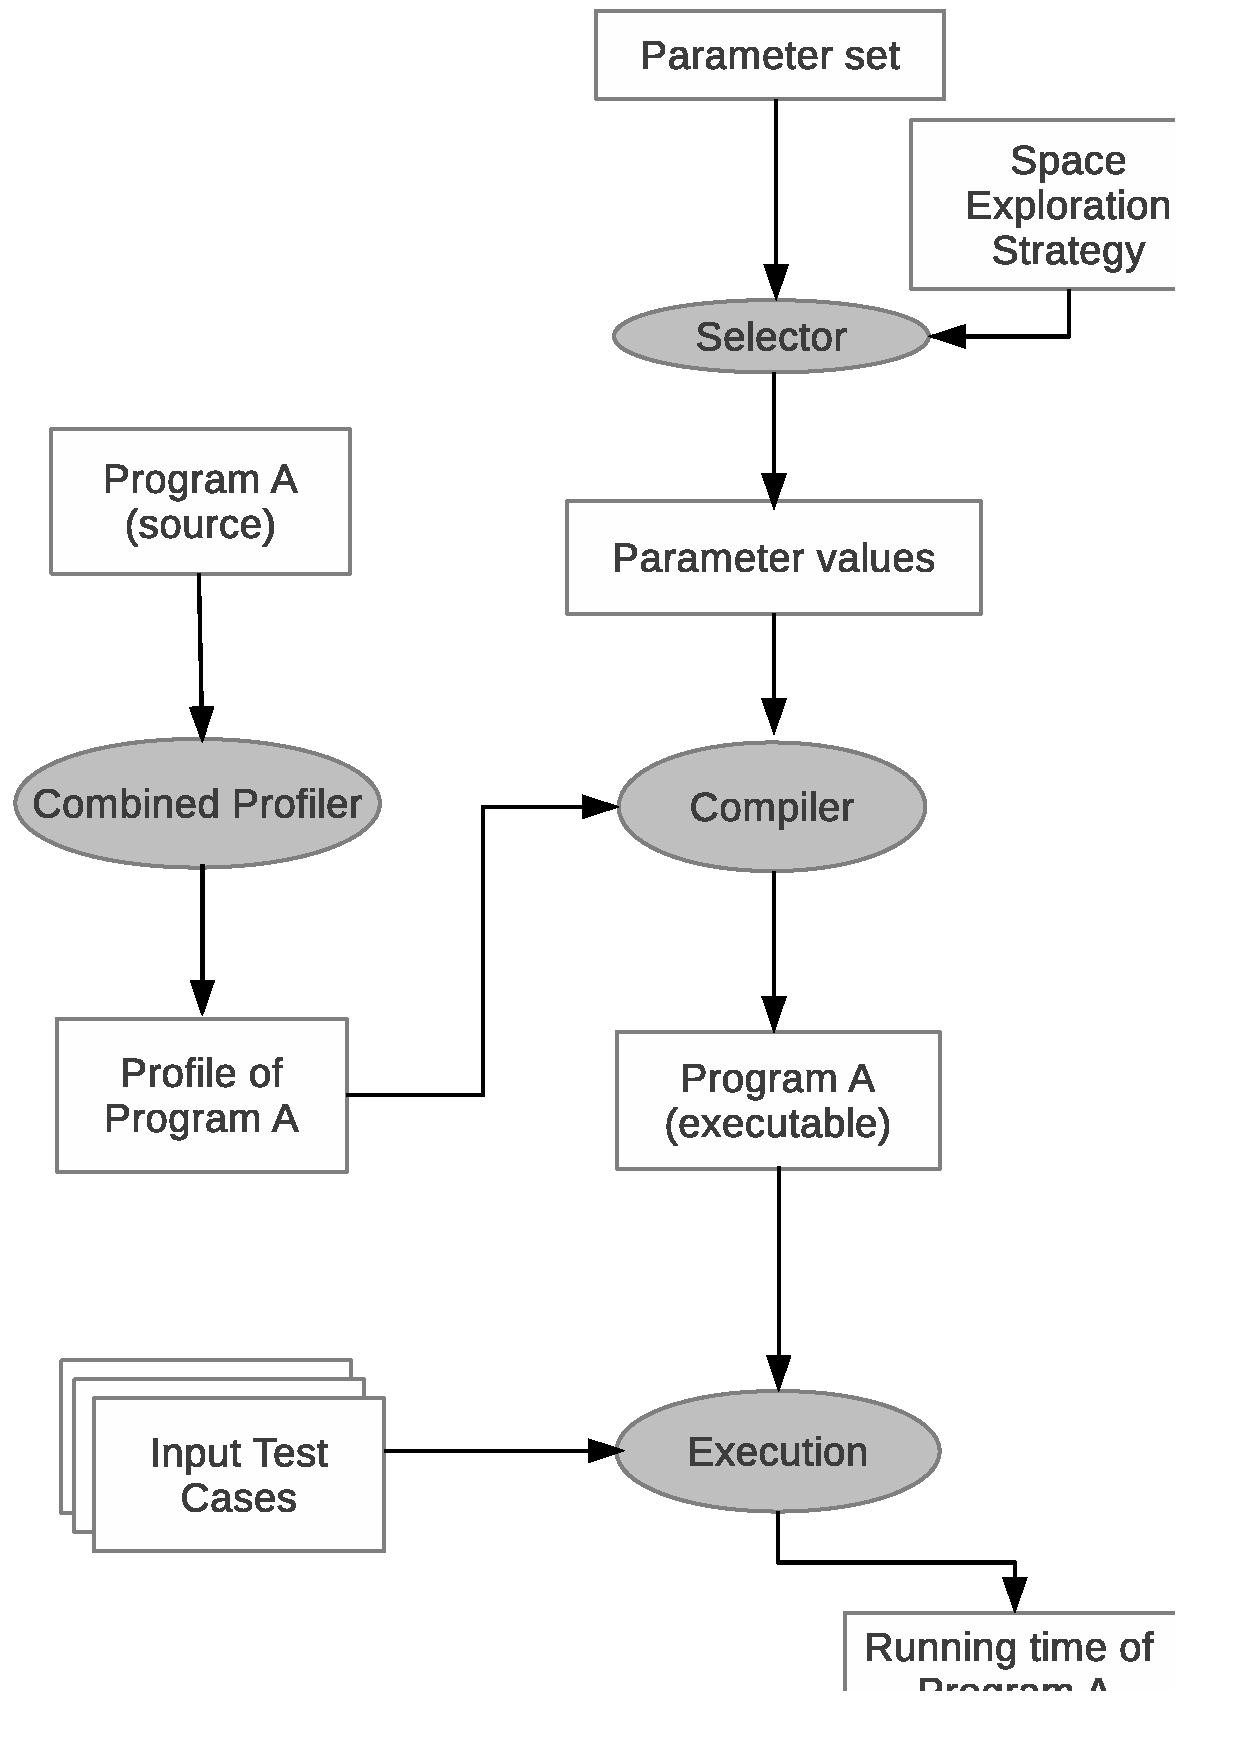
\includegraphics[width=0.50\linewidth]{Figures/genView}
  \caption{Generic view of the method}
  \label{fig:genView}
\end{figure}

We can use this method for parameter tuning, and also for a machine
learning approach trying to define the best set of parameters for
throughput or for latency. The process remains the same, we just have
to define properly what is a point of measure. More details on the
\CP\ profiling in \refFigure{fig:CPview}, whereas in \refFigure{CP:simple}
the simplified view is presented, the hatched area marks the \CP\
compiler; and in \refFigure{CP:expanded} the \CP\ compiler is shown in
more detail.

\begin{figure}
  \centering
  
  \begin{minipage}[t]{\linewidth}
    \subfigure[Simplified view of the process] {
      \begin{minipage}[b]{0.45\textwidth}
        \centering
        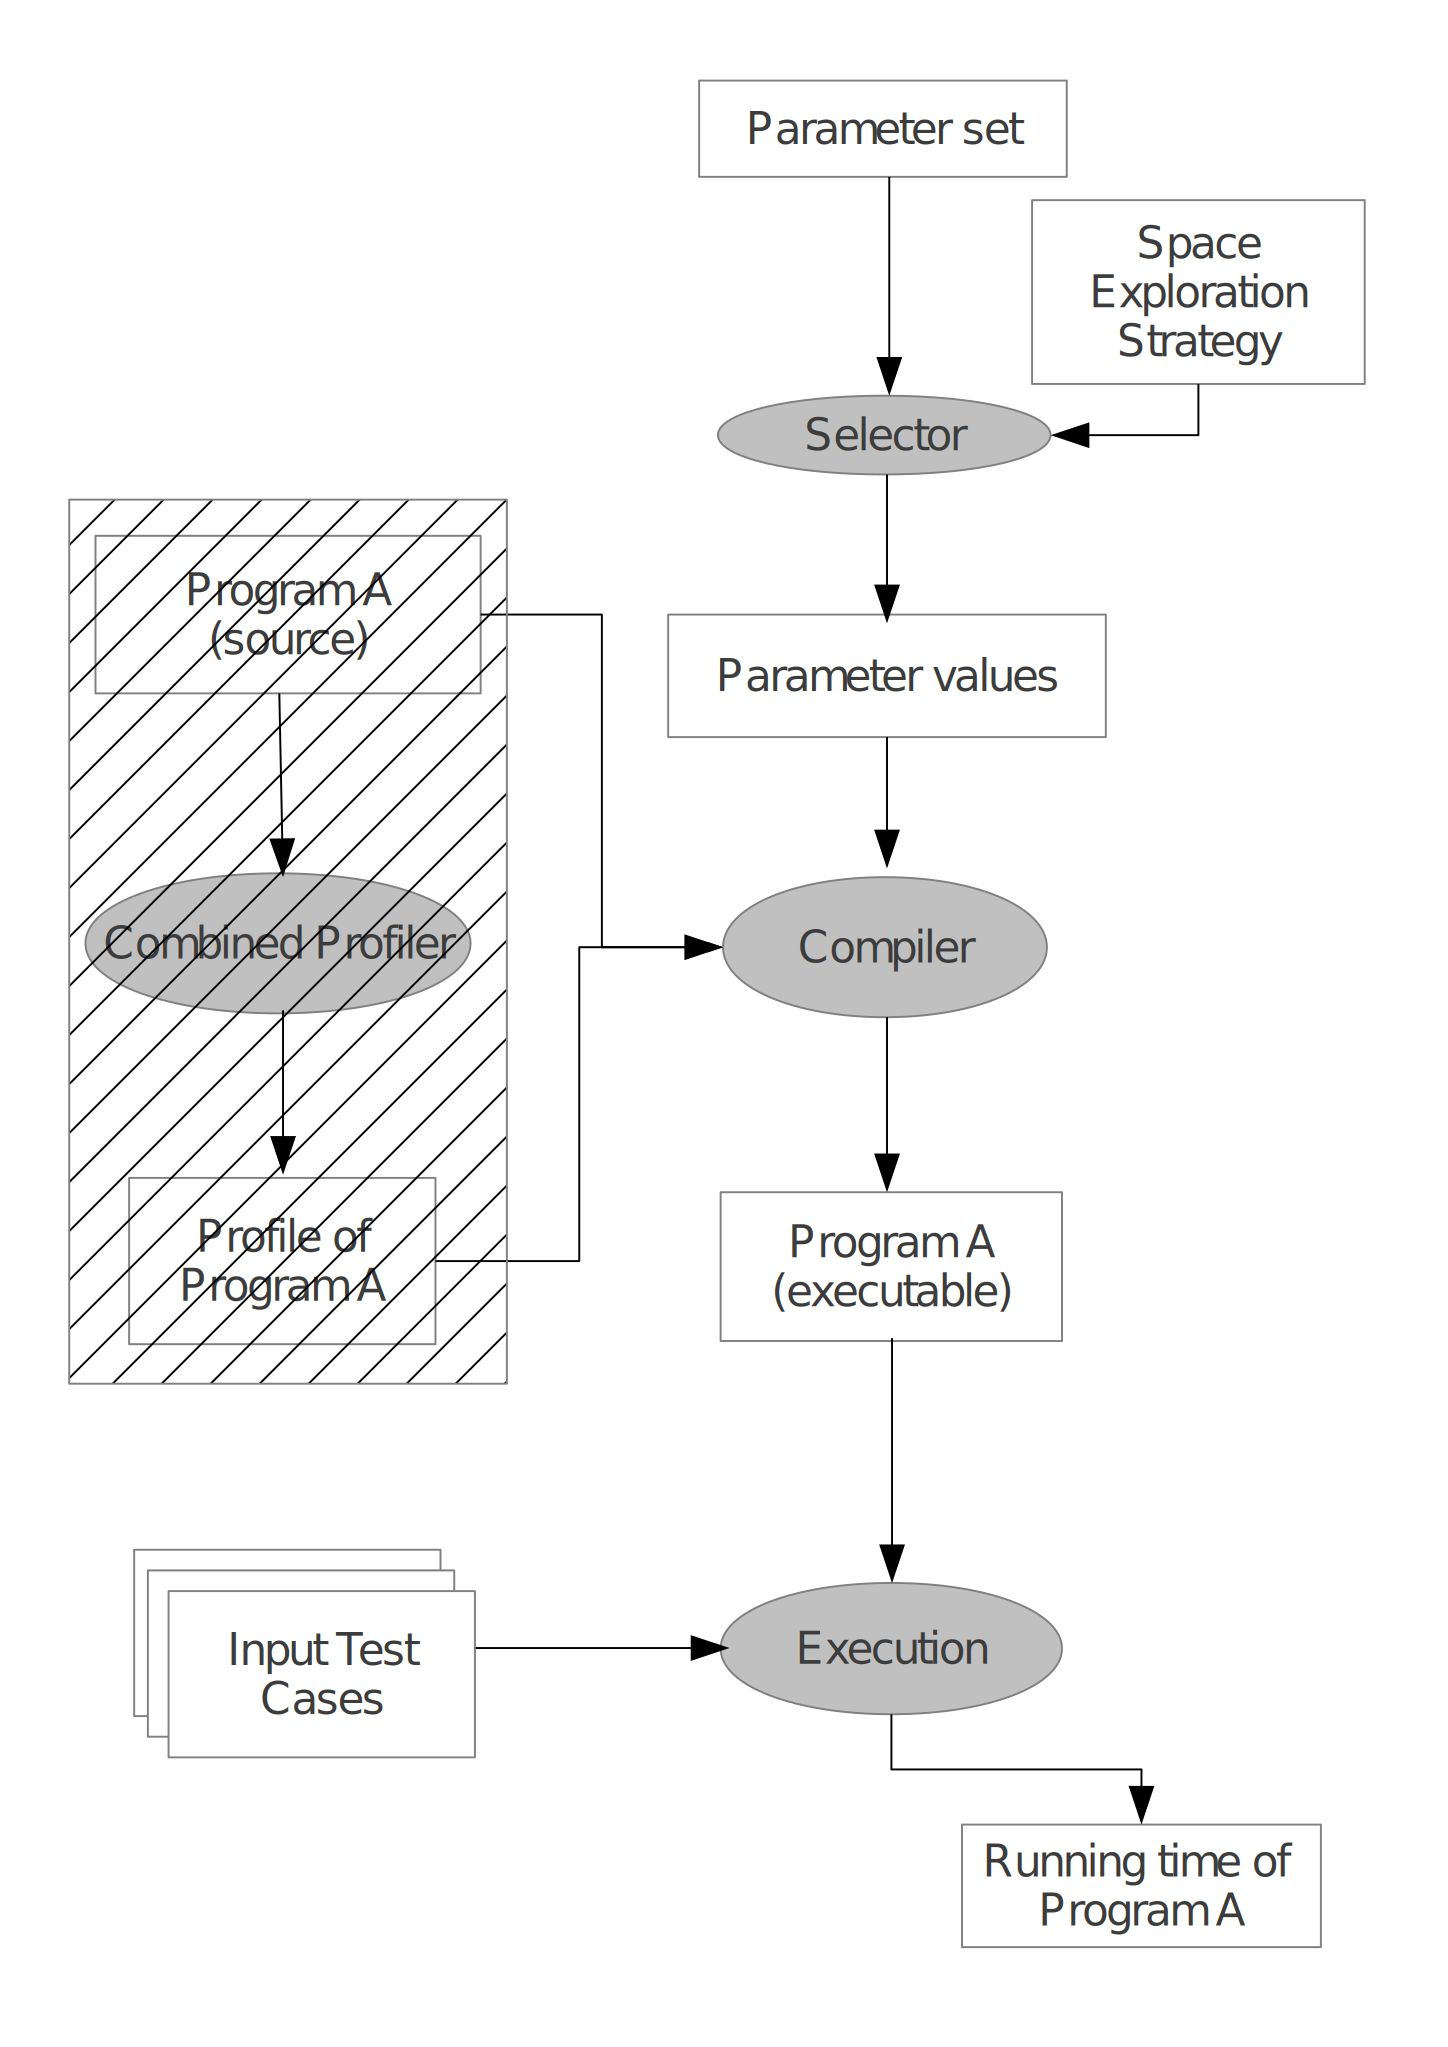
\includegraphics[height=12em]{Figures/CPview1}
      \end{minipage}
      \label{CP:simple}
    }
    \subfigure[Expanded view of the process] {
      \begin{minipage}[b]{0.45\textwidth}
        \centering
        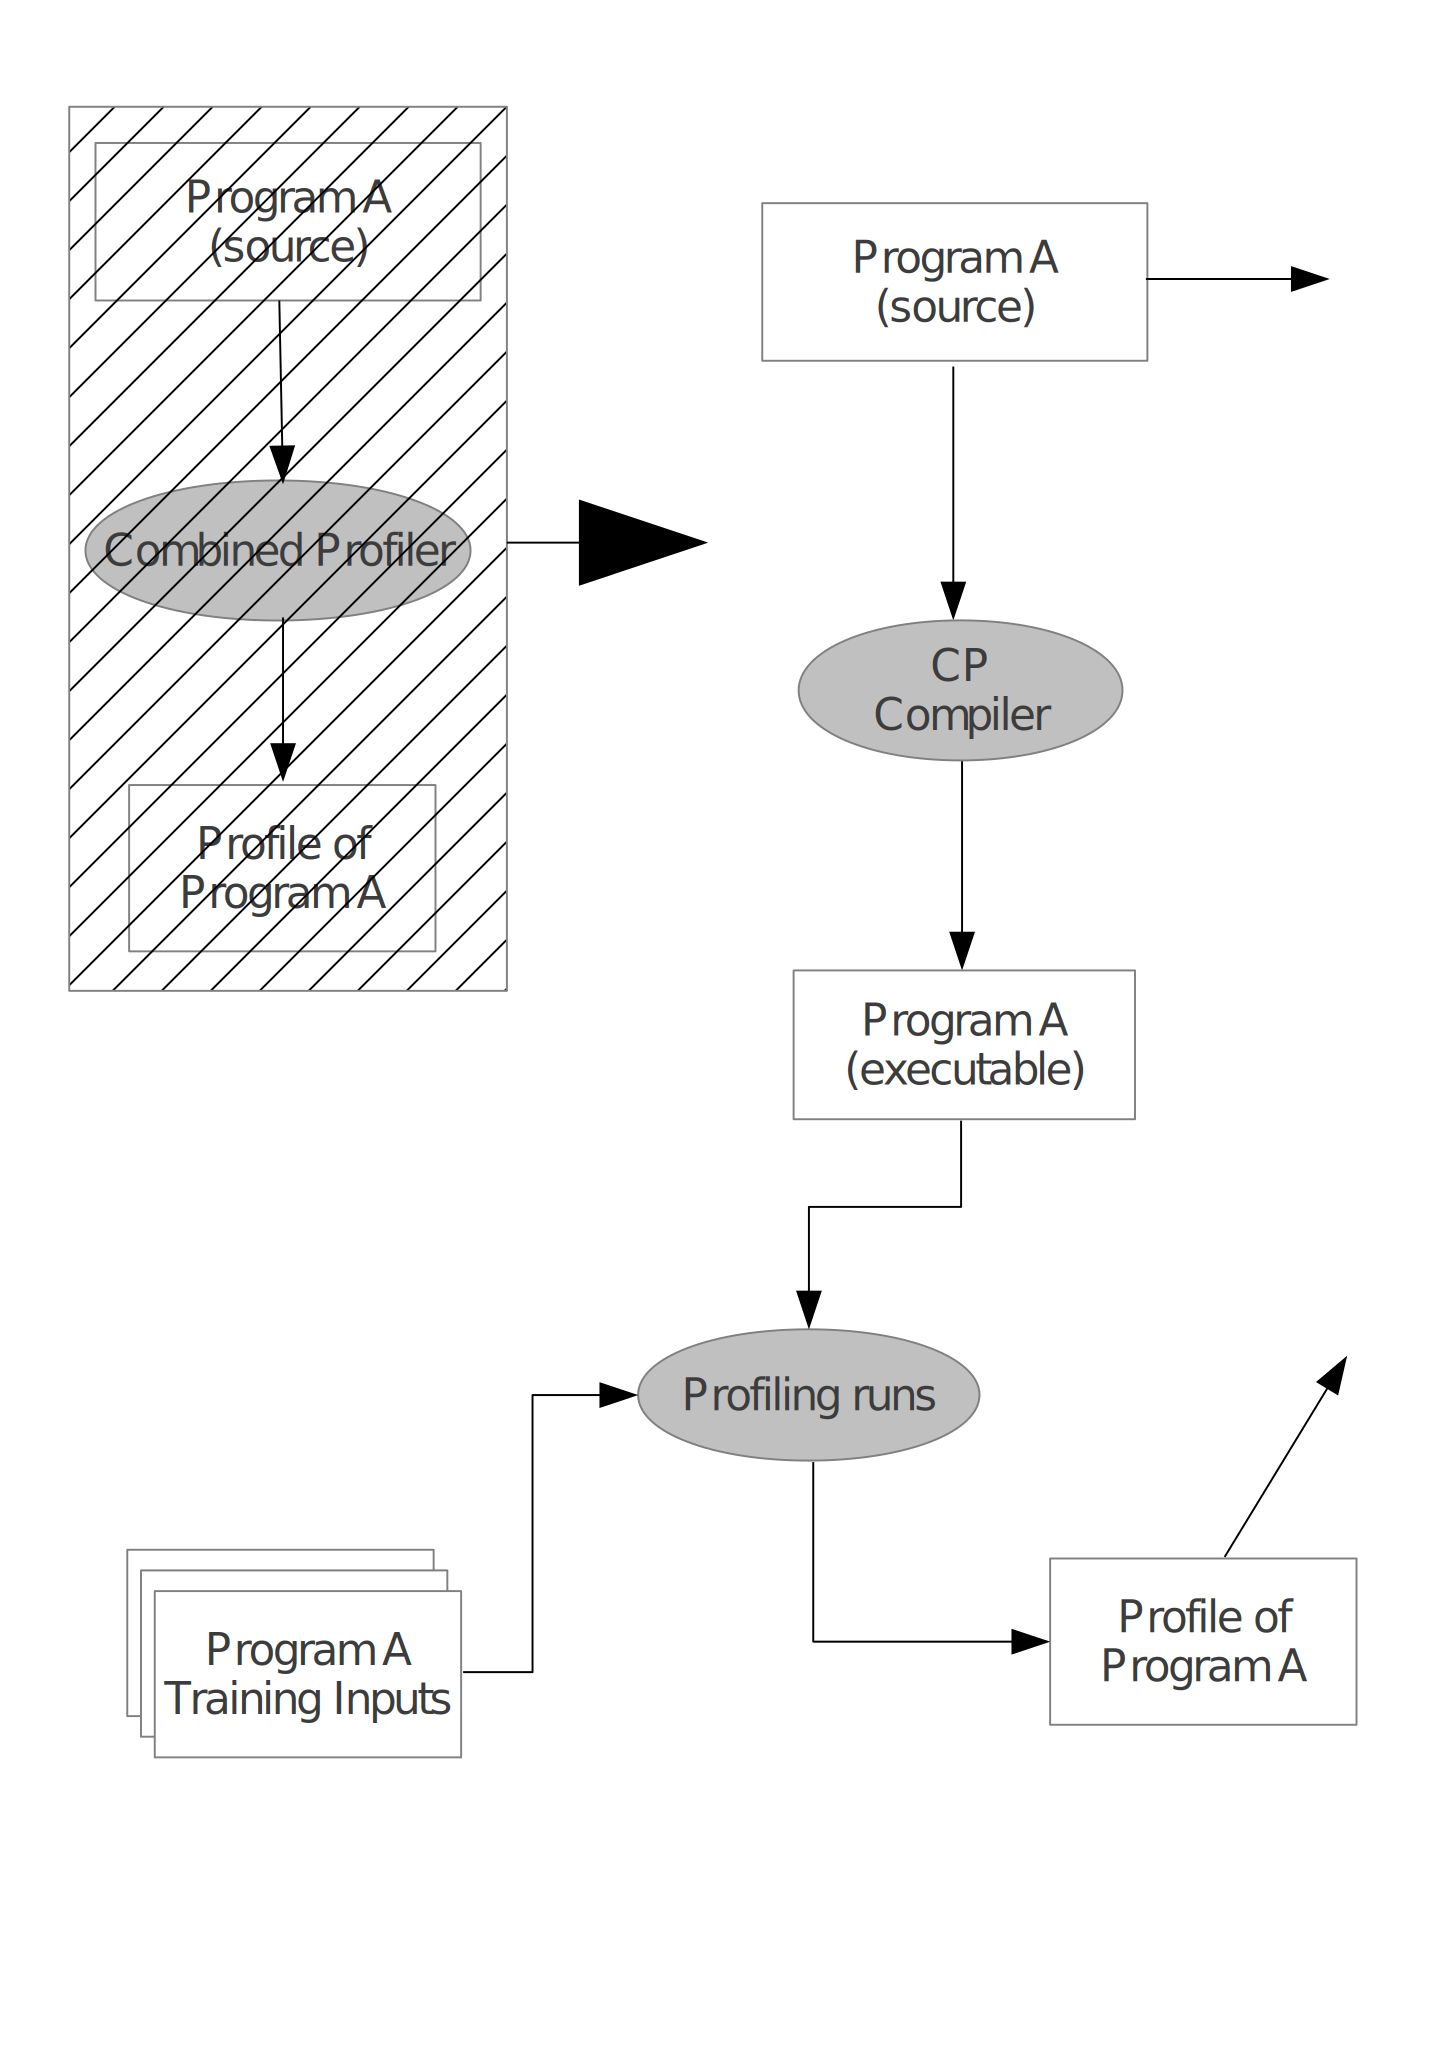
\includegraphics[height=12em]{Figures/CPview2}
      \end{minipage}
      \label{CP:expanded}
    }
    \vspace{1em}
    \hrule
    \vspace{1em}
  \end{minipage}
  \caption{\CP\ compiler and the profile generation}
  \label{fig:CPview}
\end{figure}


In the case of parameter tuning, a point of measure is represented by
the set of parameter values of the compiler for the program under tuning
and its normalized value of the execution time for some test inputs. For
the machine learning case, a point of measure for throughput is the sum
of the execution times of each of the programs under test with its
associated parameter values. On the other hand for latency, a point of
measure is the geometric mean of the normalized values.

\subsection{Parameter Tuning}

Tuning compiler optimization options for a specific program is not an easy
task \cite{Zhong2009}. There exist some tools based on Genetic Algorithms,
Simulated Anealling \cite{Zhong2009}, Support Vector Machines \cite{SanchezCGO11},
etc. For the case of inlining a recently published research pointed to the
use of Neural Networks to induce effective inlining heuristics \cite{KulkarniCGO13}.
Parameter tuning is a proficuous area of research.

As illustrated if \refFigure{fig:genView}, our method can be used effetively
to tune compiler optimization options; in this research we made an empirical
evaluation of it in the inlining case.

\section{Machine Learning Methods}
	\label{sec:ml}
	

To further characterize the problem we are facing, we need to look at
the bigger picture. We have some input points from the parameters, and
an output, the time spent by one particular program to run. And we can
compare a series of runs, with inlining, without inlining, using non-\FDO\
inlining.

With this starting point we have to define an error function and an algorithm
to search for the optimal point if it exists, or at least to get as close as
we can of it. But we don't really know any information about the space bounding
the function. We are to define and then minimize the error function on an
unknown space.

Any well known machine learning algorithm such as gradient descent
not necessarily will work properly in our environment because, as
we mentioned in ~\ref{inlining:candidate}, the function to be optimized
is not known to be differentiable nor convex. And the space that bounds
the function is also unknown.

One possible approach to this problem is to use other kinds of algorithms,
such as, Simulated Annealing \cite{Zhong2009}, or SPSA - Simultaneous Perturbation Stochastic
Approximation \cite{Spall1999,Spall2012}, because these algorithms have no
supposition on the function and on the space. They are both non-deterministic,
and make use of random points trying to avoid being trapped to a local minimum.



\section{Choice Methods}
	\label{sec:choice}
	
The scoring function, as mentioned in ~\ref{inlining:scoring} estimates the
fitness of a function to be inlined, this way a function whose score is above
zero ($0$) may be inlined, if the budget allows. But the algorithm that decides
which function will be inlined is solely based in this information, not in the
current budget value, nor in the other scores computed.

In \cite{BerubePhD} the inlining algorithm sorts the candidates for inlining
based on the score function. As the score takes into account estimated values for
benefit and cost of inlining, we suggest to use it but aggregating the expenditure,
the budget, and other scores besides the most fitted.

The idea is to perform a more compĺete version of the knapsack algorithm considering
all the scores above zero and the budget (the ``size'' of the knapsack). Proceeding
this way we can optimize the amount of budget wasted for inlining.

To make sure that there is some room for improvement in the choice of the next
function to be inlined, we are comparing the original choice (just using the highest
score) with two different ways of choosing, a random choice, and the ``more complete''
knapsack choice. Our experiments have shown that there is a best way of choosing the
candidates for the inliner, table \refTable{tab:choice} shows the results for these
three algorithms.\rr{table \refTable{tab:choice} is dummy}

\begin{table}
  \centering
  \begin{tiny}
  
\begin{tabular}{lllll}

{\bf T} & {\bf C} & {\bf Quantiles (\%)} & 
  {\bf Description} & {\bf Evaluation Name} \\ \hline

P & -- & 25 & first quartile   & QPointQ=25 \\
P & -- & 50 & estimated median & QPointQ=50 \\
P & -- & 75 & third quartile   & QPointQ=75 \\

P & L & 50, 75 & average and optimistic      & QPLinearQ=50,75 \\
P & NL   & 50, 75 &                             & QPSqrtQ=50,75   \\
P & L & 5, 95  & worst and best w/o outliers & QPLinearQ=5,95  \\
P & NL   & 5, 95  &                             & QPSqrtQ=5,95    \\

R & -- & \pair{50}{100} & top half: optimistic & QRangeQ=50,100 \\
R & -- & \pair{25}{75}  & ``central'' average  & QRangeQ=25,75  \\
R & -- & \pair{5}{95}   & average w/o outliers & QRangeQ=5,95   \\

R & L & \pair{0}{25}, \pair{75}{100} & pessimistic and optimistic
  & QRLinearQ=0,25,75,100 \\
R & NL   & \pair{0}{25}, \pair{75}{100} & 
  & QRSqrtQ=0,25,75,100 \\

\hline
\end{tabular}

  \end{tiny}
  \caption{Running time of experiments, considering $3$-times run}
  \label{tab:choice}
\end{table}

The results shown in figure \refFigure{fig:choice} refer to the geometric mean of all
the runs for each program and each input data. We have the running time for each program
in the $y$-axis, and the programs and input data on the $x$-axis. The performance of the
three different algorithms are shown for comparison.\rr{figure \refFigure{fig:choice} is dummy}

\begin{figure}
  \centering
  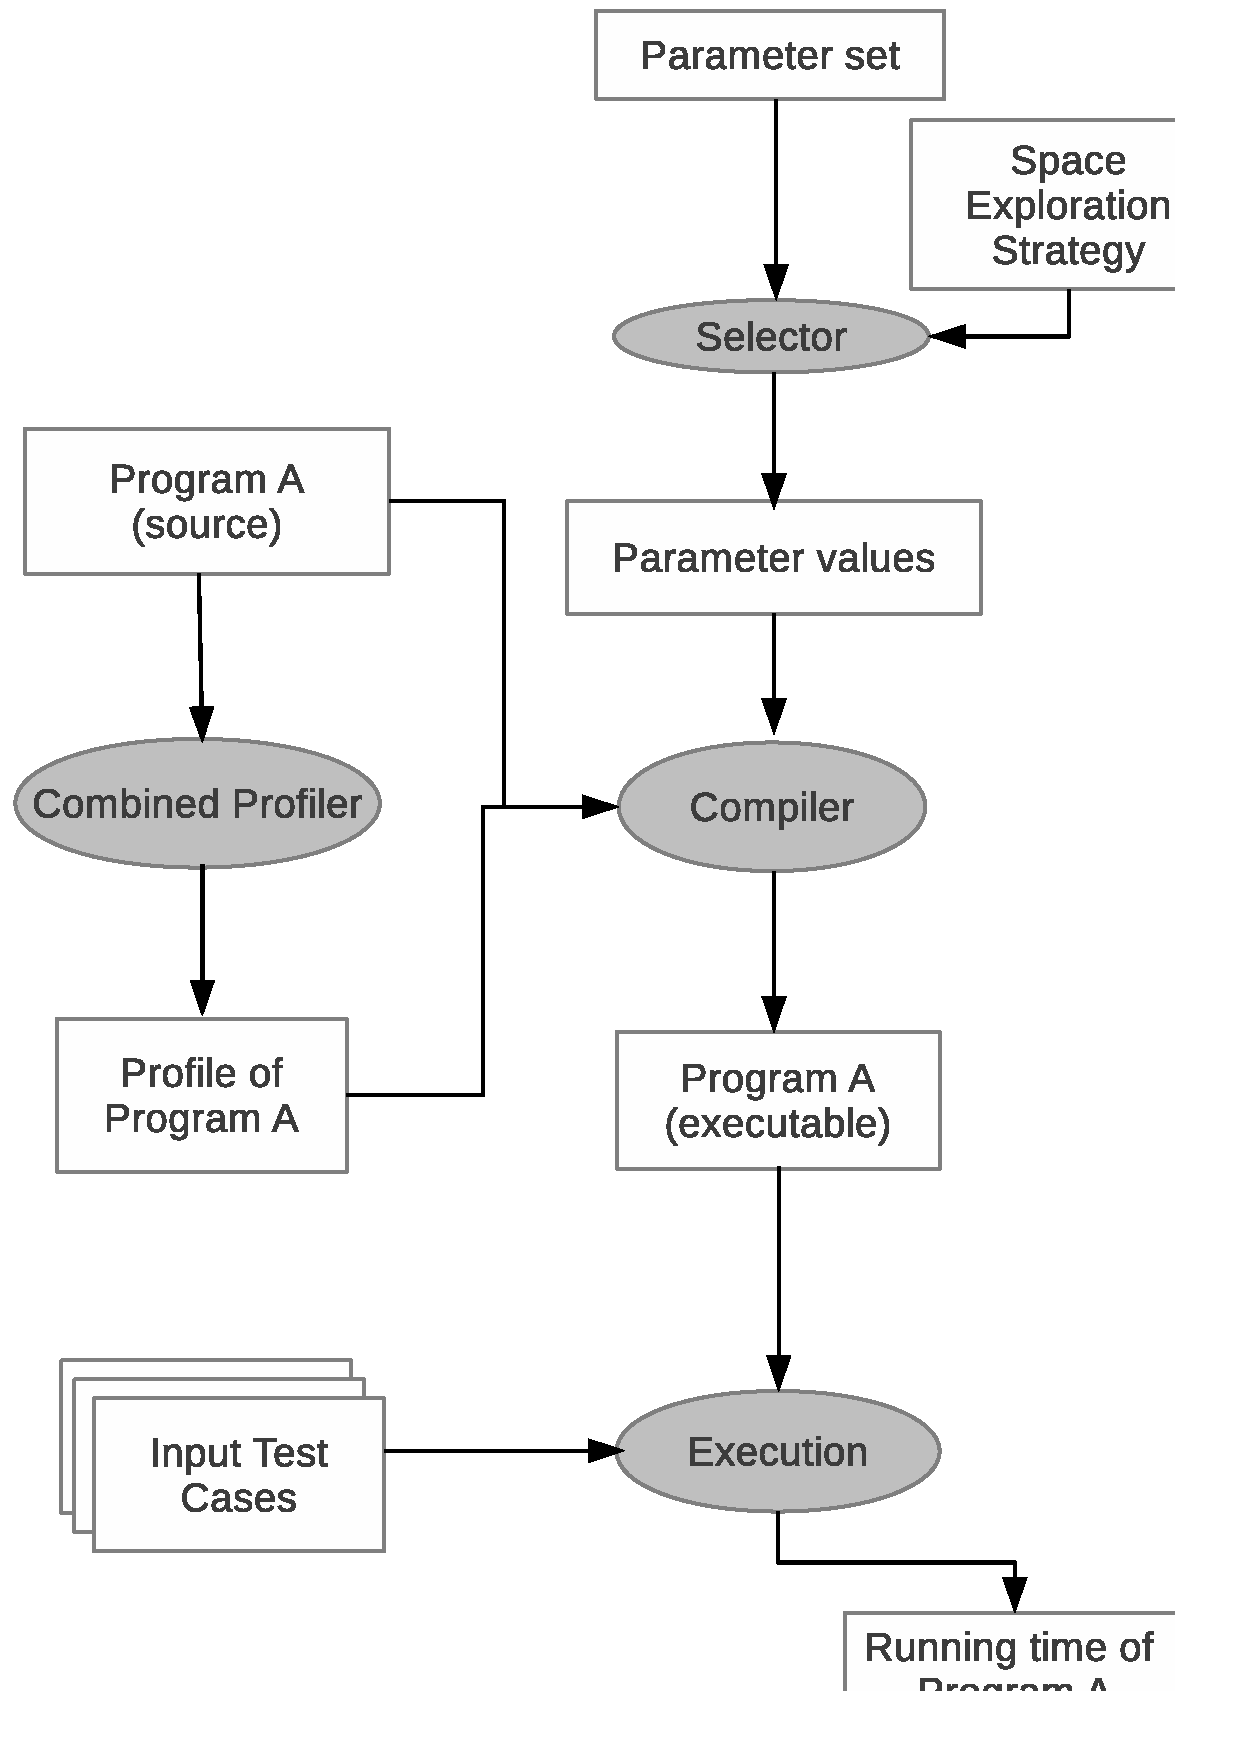
\includegraphics[width=0.50\linewidth]{Figures/choice}
  \caption{Algorithms for choosing the candidates}
  \label{fig:choice}
\end{figure}


\section{Robustness}
	\label{sec:robust}
	
To show the gaussian variation in the data we collect, figure \refFigure{fig:gauss} depicts a scatter plot of $1000$ sequential runs of the program \bzip, after being compiled using a static inliner (\llvm) whose input was {\tt ebooks}. The figure shows a gaussian noise around the median plus a few outliers, generated by the operating system regular use. These outliers are filtered off from the data we are using. They are easily discarded because they have much more variance (more than one deviation from the median).

\begin{figure}
  \centering
  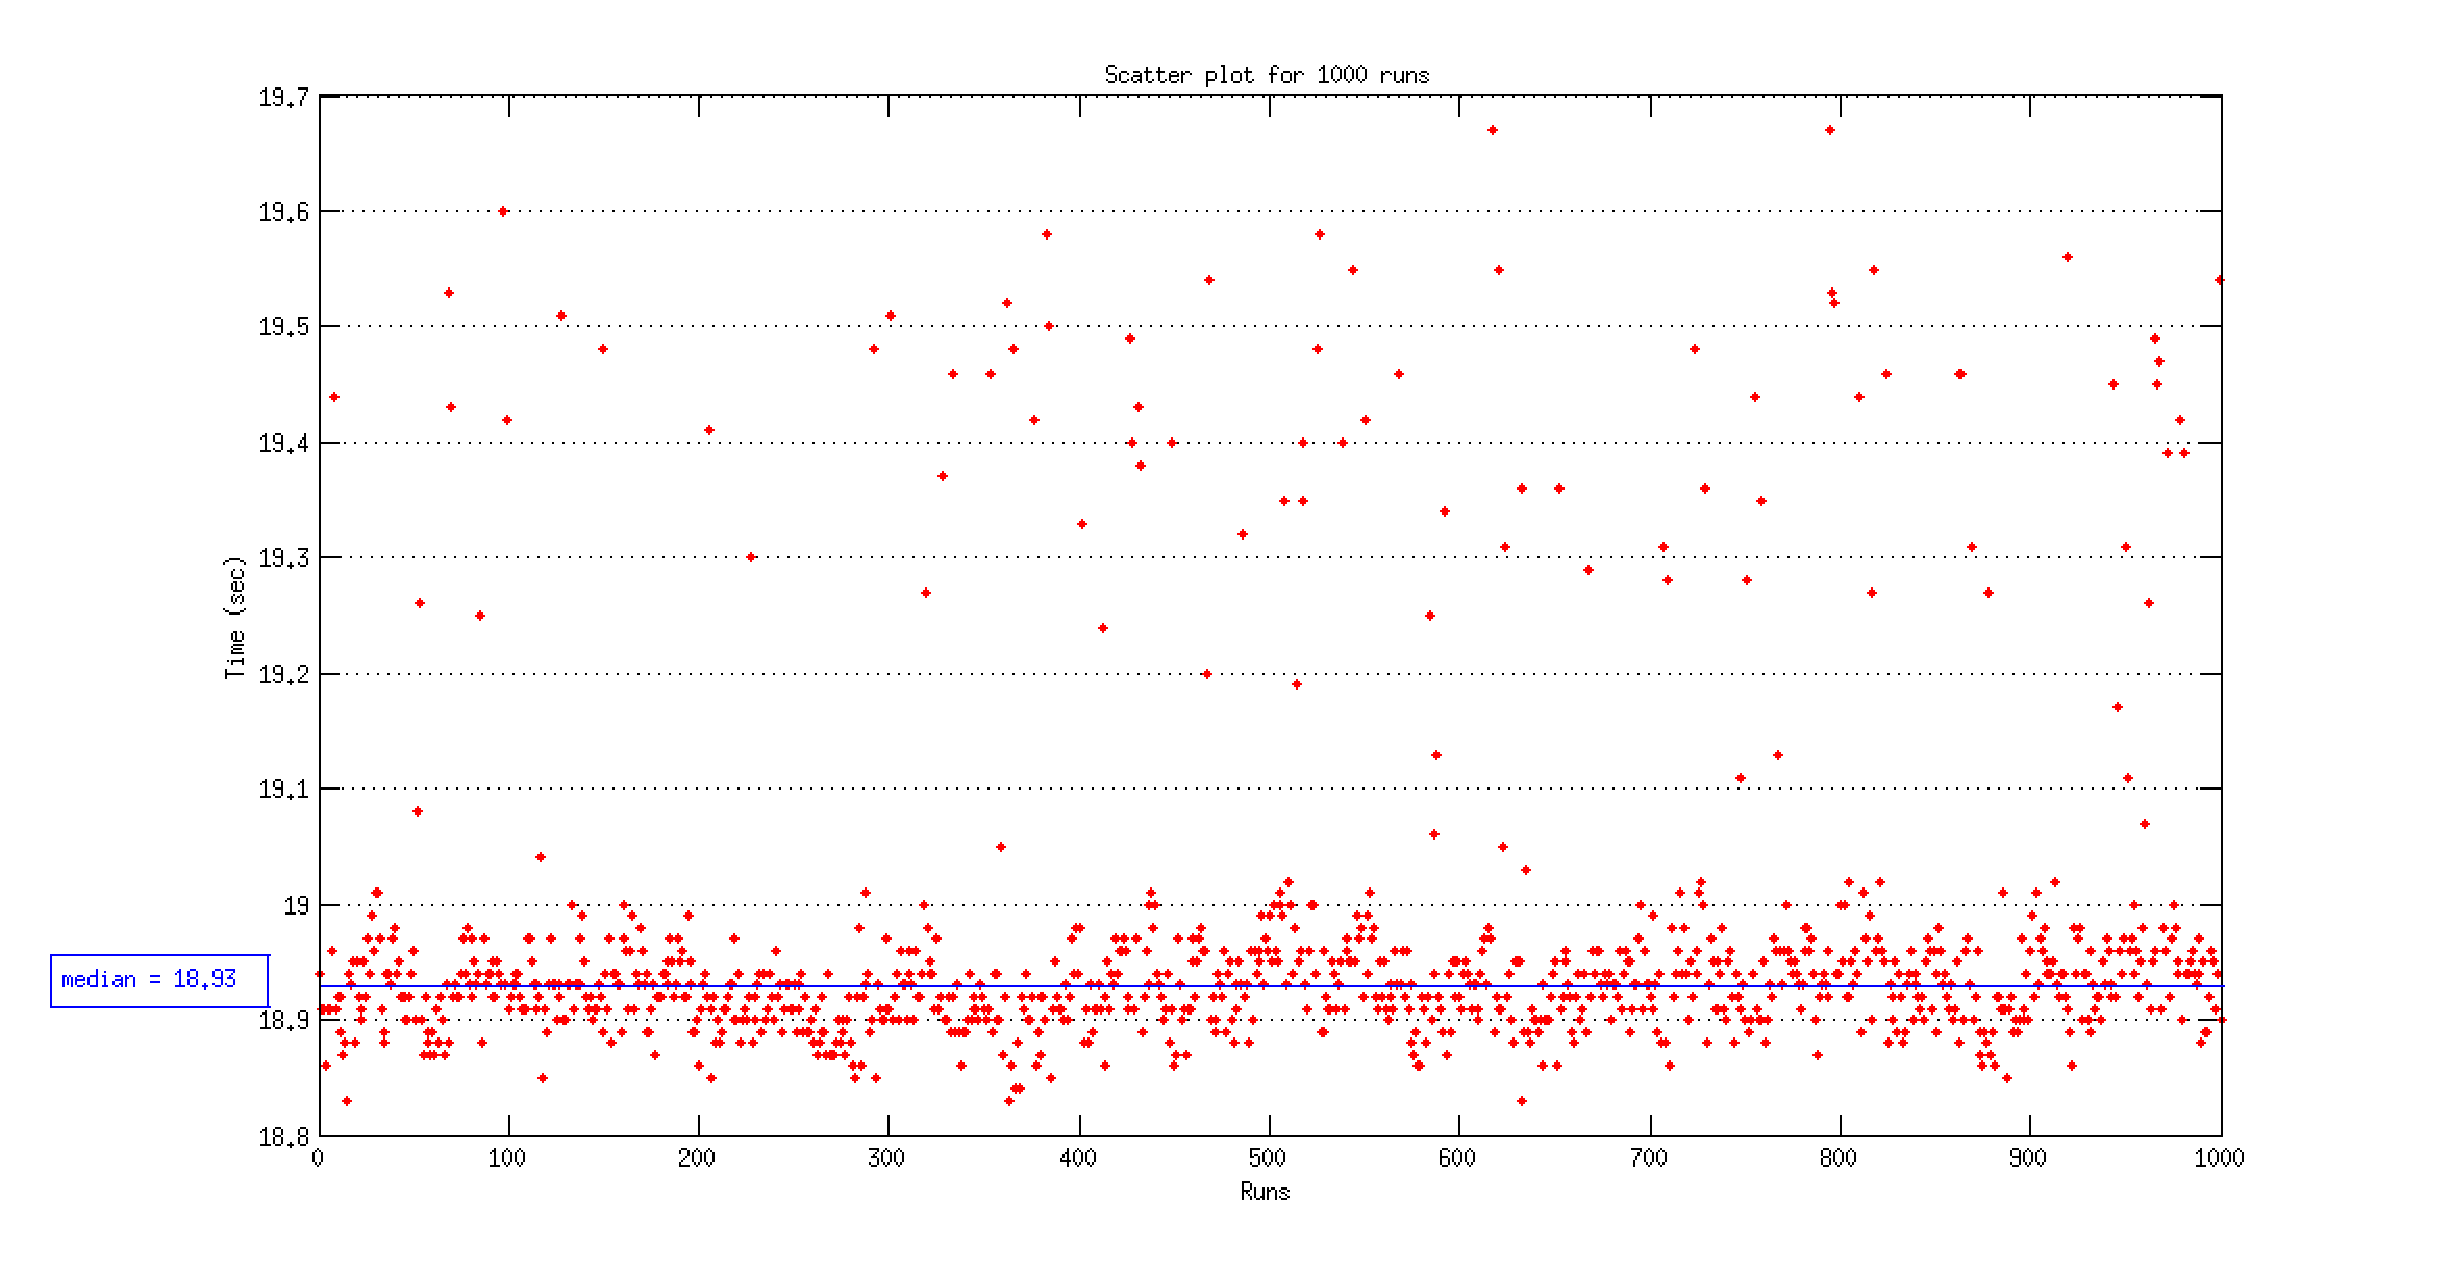
\includegraphics[width=1.00\linewidth]{Figures/1000Runs}
  \caption{Running $1000$ times the same program with the same input data}
  \label{fig:gauss}
\end{figure}

We ran three independent experiments, the first is the $10$-times experiment, then $100$-times and, after that, $1000$-times, because we needed to confirm that there is no difference on their means, and also that we can discard the outliers. To make sure that we have robust measures, we ran some simple statistics to know the mean, the median, the standard-deviation from the mean (std-mean), and the standard-deviation from the median (std-median), shown in \refTable{tab:robustTest}. We also ran t-tests on each sample pairs to verify if their means were the same, the results for the t-tests are shown in \refTable{tab:ttest} below.

\begin{table}
  \centering
  \begin{tiny}
  
\begin{tabular}{lllll}

{\bf Length} & {\bf Mean} & {\bf Median} & 
  {\bf StD Mean} & {\bf StD Median} \\ \hline

10   & 8.7160 & 8.7150 & 0.0100 & 0.0050 \\
100  & 8.7328 & 8.7200 & 0.0187 & 0.0100 \\
1000 & 8.7248 & 8.7200 & 0.0197 & 0.0100 \\

\hline
\end{tabular}

  \end{tiny}
  \caption{Simple statistics on the experiment}
  \label{tab:robustTest}
\end{table}

The t-tests in \refTable{tab:ttest} show that the null hypothesis cannot be discarded, as the value $0$ in each line of the \emph{t-test} column confirms. The \emph{p-values} illustrates the confidence in the hypothesis, in this case, that the means are different.

\begin{table}
  \centering
  \begin{tiny}
  
\begin{tabular}{lllll}

{\bf Runs} & {\bf t-test} & {\bf p-value}  \\ \hline

(10-100) & 0 & 0.3424  \\
(10-1000) & 0 & 0.6025 \\
(100-1000) & 0 & 0.1528 \\

\hline
\end{tabular}

  \end{tiny}
  \caption{t-tests applied pairwise to the $10$, $100$, and $1000$ runs}
  \label{tab:ttest}
\end{table}

\rr{Probably running 3-fold will not be enough, if the running time for a data set is much higher than the running time of this exercise, we have to expect much more noise in the data, but it will be embedded in the data, therefore impossible to extract directly. The only countermeasure is to increase the number of times we run each program from 3 to 5, maybe this could be enough.}

Our experiments have shown that the variance running the same data just three times in a row is not quite different from the $100$ times, when we consider each run a three-fold run, which means running $300$ times the same experiment. What this result means is that we empirically verified the robustness of the \CP\ methodology. As figure \refFigure{fig:CProbust} below shows, the deviation from the mean is not large (\refFigure{CP:mean}), as much as the deviation from the median (\refFigure{CP:median}).  In these figures the $y$-axis reflects the running time for each program on each input data on the $x$-axis.\rr{All other figures in this section figures are dummy}

\begin{figure}
  \centering
  
  \begin{minipage}[t]{\linewidth}
    \subfigure[Each $3$-fold mean run compared with the $300$-times run mean] {
      \begin{minipage}[b]{0.45\textwidth}
        \centering
        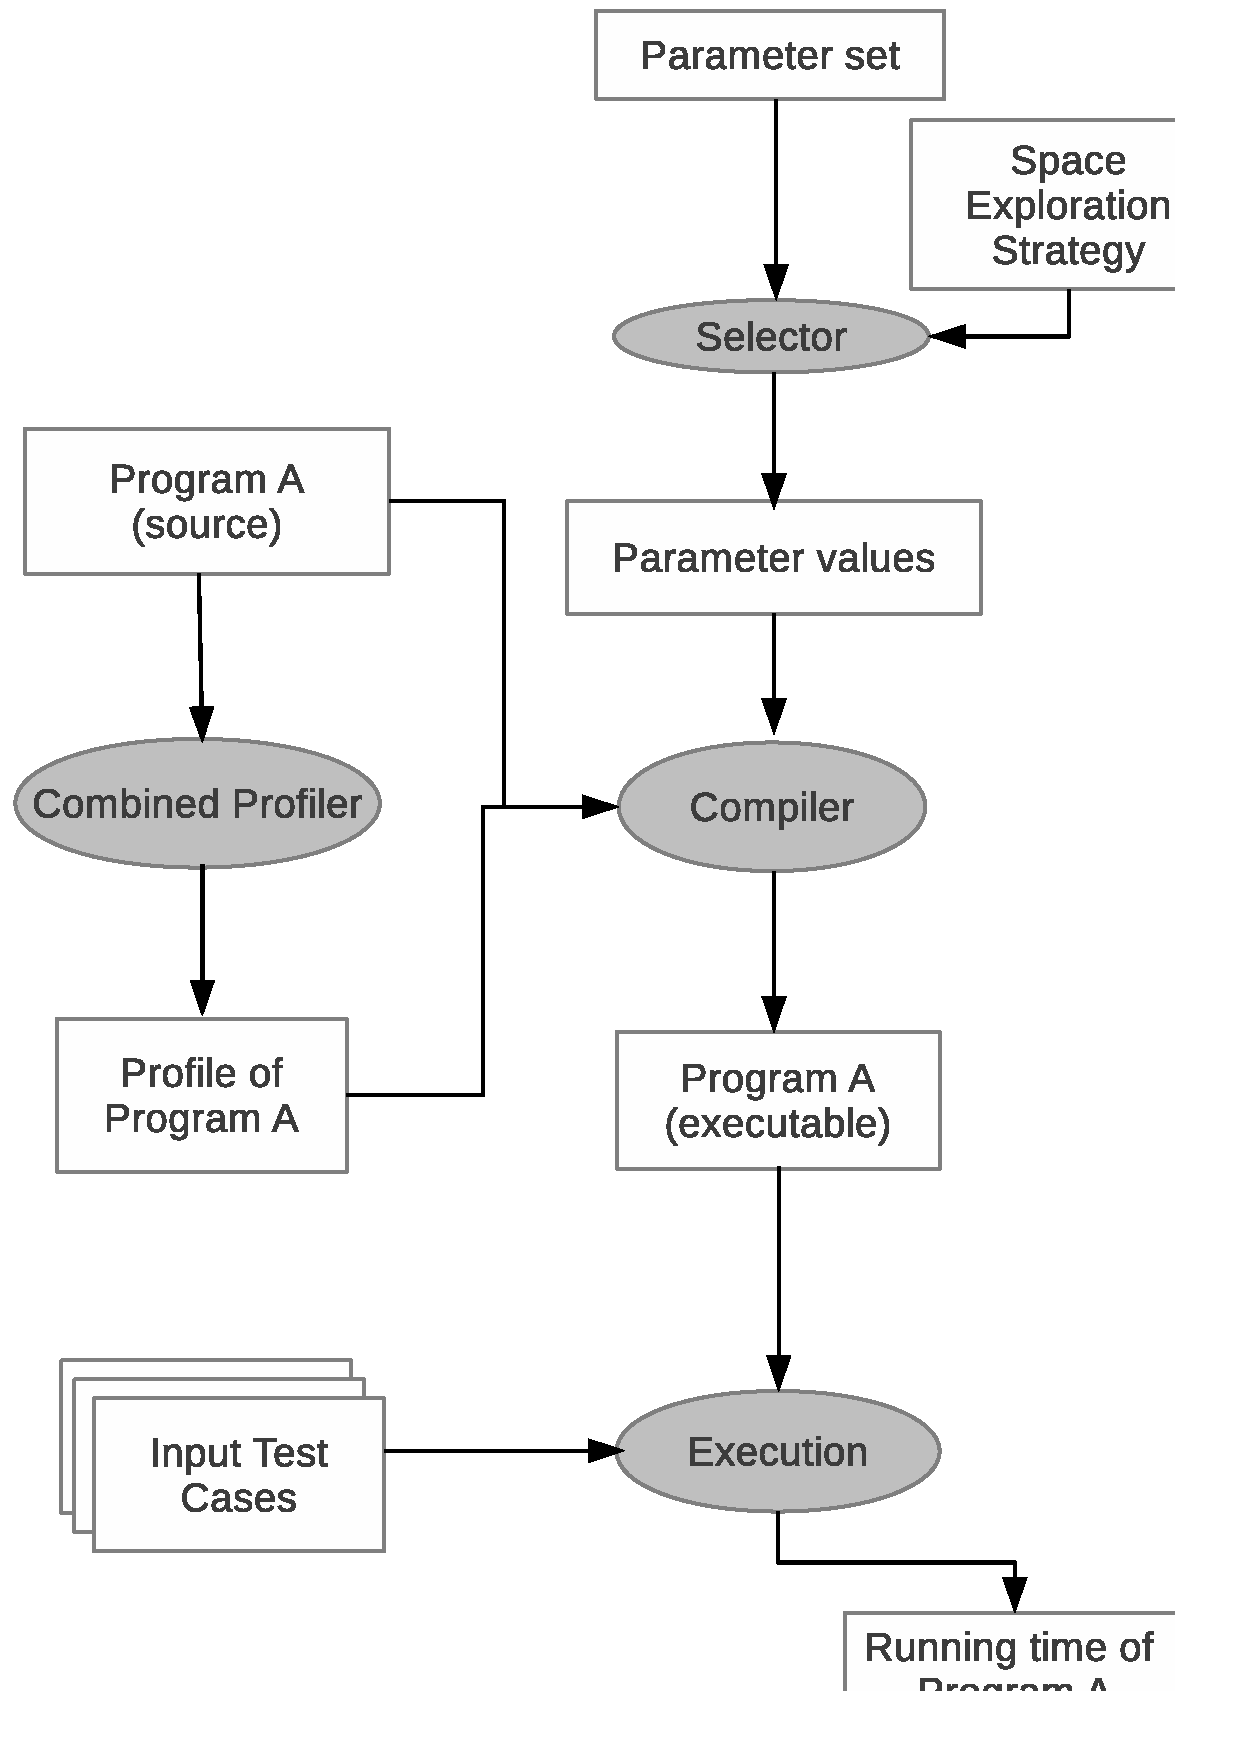
\includegraphics[height=12em]{Figures/CPmean}
      \end{minipage}
      \label{CP:mean}
    }
    \subfigure[Each $3$-fold median run compared with the $300$-times run median] {
      \begin{minipage}[b]{0.45\textwidth}
        \centering
        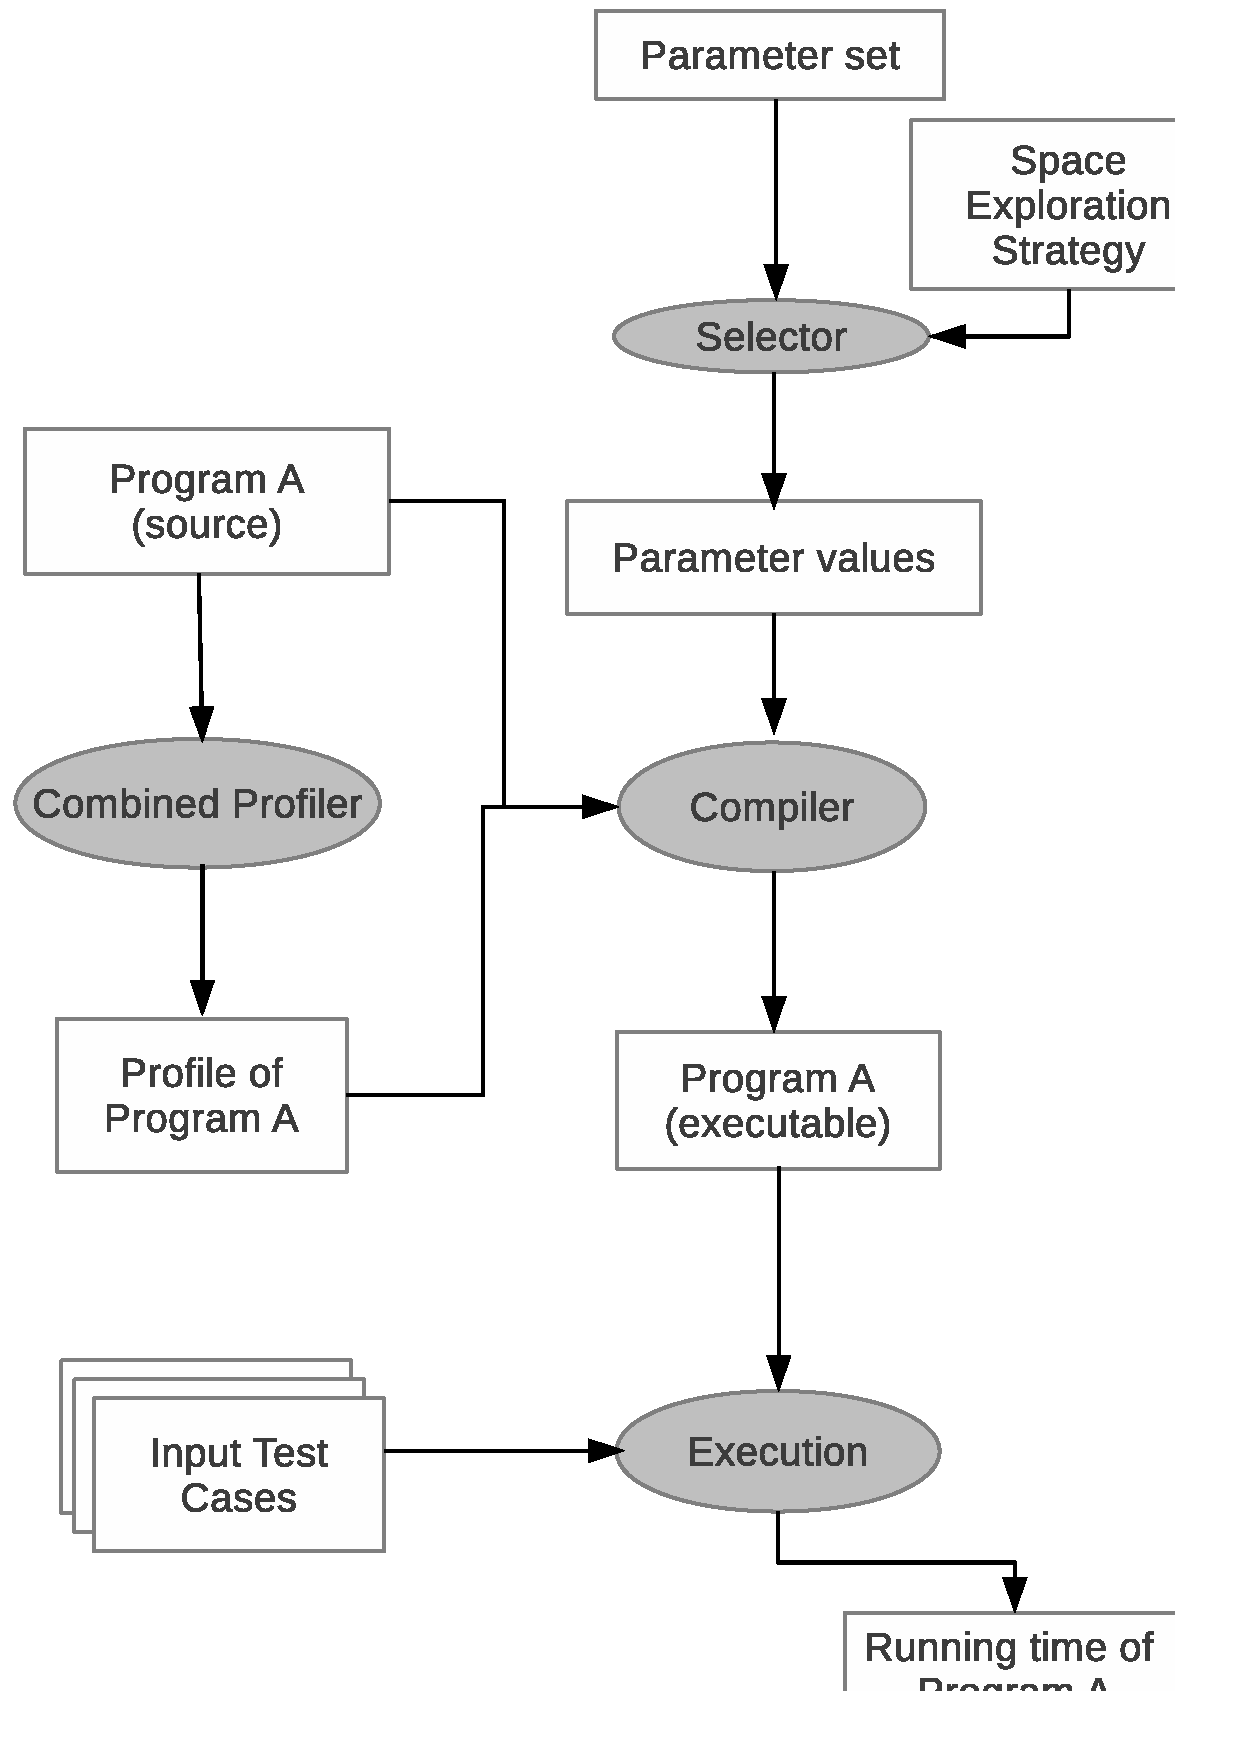
\includegraphics[height=12em]{Figures/CPmedian}
      \end{minipage}
      \label{CP:median}
    }
  \end{minipage}
  \caption{$100$-times running $3$-times experiment}
  \label{fig:CProbust}
\end{figure}

The data used in the experiment are shown in \refTable{tab:simStats}, and the deviations from the mean (and median) to each $3$-fold run are summarized as the average, minimum, and maximum values, all found on the $300$-times experiment.\rr{All other tables in this section figures are dummy}

\begin{table}
  \centering
  \begin{tiny}
  
\begin{tabular}{lllll}

{\bf Run} & {\bf Mean} & {\bf Median} & 
  {\bf StD Mean} & {\bf StD Median} \\ \hline

1 & 8.7233 & 8.72 & 0.0044   \\
2 & 8.71 & 8.71 & 0.0067 & 0.01   \\
3 & 8.72 & 8.73 & 0.02 & 0.01   \\
4 & 8.7067 & 8.7 & 0.0089 & 0.00   \\
5 & 8.71 & 8.71 & 0.0067 & 0.01   \\
6 & 8.7933 & 8.74 & 0.0778 & 0.01   \\
7 & 8.73 & 8.73 & 0.0067 & 0.01   \\
8 & 8.7233 & 8.71 & 0.0178 & 0.00   \\
9 & 8.73 & 8.73 & 0.0067 & 0.01   \\
10 & 8.7033 & 8.71 & 0.0089 & 0.00   \\
\\
33 & 8.71 & 8.71 & 0.0067 & 0.01   \\
34 & 8.7267 & 8.73 & 0.0044 & 0.00   \\
35 & 8.71 & 8.7 & 0.0133 & 0.00   \\
36 & 8.81 & 8.73 & 0.1133 & 0.01   \\
37 & 8.72 & 8.72 & 0.0133 & 0.02   \\
\\
70 & 8.72 & 8.71 & 0.0133 & 0.00   \\
71 & 8.7133 & 8.72 & 0.0089 & 0.00   \\
72 & 8.7233 & 8.72 & 0.0044 & 0.00   \\
73 & 8.7233 & 8.72 & 0.0044 & 0.00   \\
74 & 8.743333 & 8.74 & 0.0111 & 0.01   \\
75 & 8.7667 & 8.76 & 0.0156 & 0.01   \\
76 & 8.7967 & 8.8 & 0.0111 & 0.01   \\
77 & 8.8133 & 8.82 & 0.0089 & 0.00   \\
78 & 8.83 & 8.83 & 0.0067 & 0.01   \\
79 & 8.8433 & 8.84 & 0.0111 & 0.01   \\
80 & 8.74 & 8.74 & 0 & 0.00   \\
81 & 8.7833 & 8.78 & 0.0111 & 0.01   \\
82 & 8.77 & 8.77 & 0.0067 & 0.01   \\
83 & 8.7667 & 8.76 & 0.0222 & 0.02   \\
84 & 8.79 & 8.79 & 0.0067 & 0.01   \\
85 & 8.7633 & 8.76 & 0.0044 & 0   \\
86 & 8.7533 & 8.76 & 0.0156 & 0.01   \\
87 & 8.7467 & 8.74 & 0.0089 & 0.00   \\
88 & 8.74 & 8.74 & 0.0067 & 0.01   \\
89 & 8.7567 & 8.76 & 0.0111 & 0.01   \\
90 & 8.7267 & 8.72 & 0.0156 & 0.01   \\
91 & 8.71 & 8.71 & 0.0067 & 0.01   \\
\\
92 & 8.7133 & 8.71 & 0.0044 & 0   \\
93 & 8.79 & 8.75 & 0.0733 & 0.03   \\
94 & 8.7167 & 8.72 & 0.0044 & 0   \\
95 & 8.72 & 8.71 & 0.0133 & 0   \\
96 & 8.73 & 8.73 & 0.00 & 0.00   \\
97 & 8.73 & 8.74 & 0.02 & 0.01   \\
98 & 8.73 & 8.74 & 0.02 & 0.01   \\
99 & 8.7133 & 8.72 & 0.0089 & 0   \\
100 & 8.7367 & 8.74 & 0.0178 & 0.02   \\

\hline
\end{tabular}

  \end{tiny}
  \caption{Deviation from the mean and from the median in the experiment}
  \label{tab:simStats}
\end{table}

We also ran the t-tests to show that the means (and the medians) are statistically representing the same distribution. This is summarized in \refTable{tab:statTest} below.

\begin{table}
  \centering
  \begin{tiny}
  
\begin{tabular}{lllll}

{\bf T} & {\bf C} & {\bf Quantiles (\%)} & 
  {\bf Description} & {\bf Evaluation Name} \\ \hline

P & -- & 25 & first quartile   & QPointQ=25 \\
P & -- & 50 & estimated median & QPointQ=50 \\
P & -- & 75 & third quartile   & QPointQ=75 \\

P & L & 50, 75 & average and optimistic      & QPLinearQ=50,75 \\
P & NL   & 50, 75 &                             & QPSqrtQ=50,75   \\
P & L & 5, 95  & worst and best w/o outliers & QPLinearQ=5,95  \\
P & NL   & 5, 95  &                             & QPSqrtQ=5,95    \\

R & -- & \pair{50}{100} & top half: optimistic & QRangeQ=50,100 \\
R & -- & \pair{25}{75}  & ``central'' average  & QRangeQ=25,75  \\
R & -- & \pair{5}{95}   & average w/o outliers & QRangeQ=5,95   \\

R & L & \pair{0}{25}, \pair{75}{100} & pessimistic and optimistic
  & QRLinearQ=0,25,75,100 \\
R & NL   & \pair{0}{25}, \pair{75}{100} & 
  & QRSqrtQ=0,25,75,100 \\

\hline
\end{tabular}

  \end{tiny}
  \caption{Test on the means and medians}
  \label{tab:statTest}
\end{table}

This experiment brought us confidence in the machine learning method we devised to tune-in the compiler parameters. We considered the possibility of increasing the number of times each individual run need to be performed, in order to achieve low variance in the data; hence we could trust the results. As this experiment has shown, the $3$-fold run is a good choice, because it does not penalize much the total running time. We show these data in \refTable{tab:runTime}.

\begin{table}
  \centering
  \begin{tiny}
  
\begin{tabular}{lllll}

{\bf T} & {\bf C} & {\bf Quantiles (\%)} & 
  {\bf Description} & {\bf Evaluation Name} \\ \hline

P & -- & 25 & first quartile   & QPointQ=25 \\
P & -- & 50 & estimated median & QPointQ=50 \\
P & -- & 75 & third quartile   & QPointQ=75 \\

P & L & 50, 75 & average and optimistic      & QPLinearQ=50,75 \\
P & NL   & 50, 75 &                             & QPSqrtQ=50,75   \\
P & L & 5, 95  & worst and best w/o outliers & QPLinearQ=5,95  \\
P & NL   & 5, 95  &                             & QPSqrtQ=5,95    \\

R & -- & \pair{50}{100} & top half: optimistic & QRangeQ=50,100 \\
R & -- & \pair{25}{75}  & ``central'' average  & QRangeQ=25,75  \\
R & -- & \pair{5}{95}   & average w/o outliers & QRangeQ=5,95   \\

R & L & \pair{0}{25}, \pair{75}{100} & pessimistic and optimistic
  & QRLinearQ=0,25,75,100 \\
R & NL   & \pair{0}{25}, \pair{75}{100} & 
  & QRSqrtQ=0,25,75,100 \\

\hline
\end{tabular}

  \end{tiny}
  \caption{Running time of experiments, considering $3$-times run}
  \label{tab:runTime}
\end{table}

If we had to run more than three times, say $n$ times, the total running time would be increased for a factor of $k$, where $k = \frac{n}{3}$, which, in case $n = 9$, would result in three times the total running time we had in this experiment.


\section{Results}
	\label{sec:results}
	
\def\graphwidth{0.9\linewidth}


\REM{ % irrlelvent!
running at 2000Mhz, with 128KB L1, 512KB L2, 2MB L3 shared, and 4 GB
of memory.
}

The first experiment was to tune in the value of the compiler parameters.
 A machine learning algorithm was used to find the sweetspot for a set of
 inlining parameters. As described in Section~\ref{sec:ml}, we used
 SPSA - Simultaneous Perturbation Stochastic Approximation because we have no
 supposition on the function and on the search space.

The second experiment was performed to evaluate and compare two different cases,
 the case of single-runs, and the case of \CP\-runs. Both cases are analyzed and
 compared.

The third experiment was conducted to verify and 
  analyze behavior variability for random choice, simple sort and
  a version of the knapsack problem. Particularly the latter version presented better results.

\subsection{Programs and Inputs}


This study evaluates the inliners described above using four
programs: \bzip, \gzip, \gcc, and \gobmk.  Each program is evaluated
using a 15-input workload, as suggested
in \cite{BerubePhD}.  \Gcc\ and \gobmk\ are taken from the
SPEC CPU 2006 benchmark suite.  SPEC provides 11 inputs for \gcc.  In
spite of the challenges involved in creating new inputs for this
benchmark, four\footnote{of seven attempts} of the SPEC 2000 benchmark
programs were converted to the single pre-processed file format.  The
converted programs are \bzip, \lbm, \mcf, and \parser.  For \gobmk,
SPEC provides 20 inputs.  However, only 5 of these inputs come from
the {\tt ref} workload; the {\tt train} workload contains 8 inputs,
and the {\tt test} workload contains 7 inputs.  Many of the inputs from
{\tt test} and {\tt train} have very short execution times: 4 inputs
take less than 1 second, 6 take 2--9 seconds, 4 take 12--19 seconds,
and 1 takes longer than 1 minute.  Execution times of less than a few
seconds are subject to large proportional timing imprecision, because
the Linux {\tt time} command reports times with a resolution of
1/100$^{th}$ of a second.  Therefore, the 15 longest-running inputs
are chosen for \Wfull.  This set is composed of the {\tt ref} and {\tt
train} SPEC workloads, plus \iname{connect} and \iname{dniwog} from
{\tt test}.  The shortest baseline running time in \Wfull\ is 2.3
seconds, for \iname{connect}.

The other two programs used in the case study are \bzip\ and \gzip.
However, rather than using the SPEC benchmark versions of these
programs, the fully-functional ``real'' versions are used.  Using the
real versions of the compressor programs eliminates the
unrealistically-simplified profiling situation where
mutually-exclusive use cases are combined into a single program run.
Consequently, these programs cannot do decompression and compression,
or multiple levels of compression, within the same run.  These
distinct use-cases must be covered by different inputs in the program
workload.  Both \bzip\ and \gzip\ share the same workload of inputs.
This workload is split in half into a compression set and a
decompression set.  Several inputs in the compression set have an
analogue in the decompression set.  However, the file format is
usually different, and the source of the data is never the same.  For
instance, \iname{revelation\mbox{-}ogg} in the compression set
and \iname{sherlock\mbox{-}mp3} in the decompression set are both audio
books, but the audio is recorded in different formats, and the books
themselves are different.

Both compressors use a numeric command-line flag to control the
tradeoff between compression speed and compression quality.  The flags
take integer values between 1 (fastest, least compressed) and 9
(slowest, most compressed).  The seven inputs in the compression set
each use a different compression level, from 3 to 9.  Most inputs are
collections of files.  Each collection is archived (uncompressed) so
that the input and output of each run is a single file.  In order to
minimize the impact of disk access, the output of each run is
redirected to {\tt /dev/null}.

The compression set contains the following inputs, with the
compression level shown in parentheses:
\begin{itemize}

\item {\tt avernum (-3)}: The installer for the demo version of the game
  ``Avernum: Escape from the Pit'' from Spiderweb Software.

\item {\tt cards (-4)}: A collection of greeting card layouts in the TIFF 
  (uncompressed) image format.

\item {\tt ebooks (-5)}: A collection of ebooks, with and without images,
  and in a variety of formats, from Project
  Gutenberg\footnote{http://www.gutenberg.org}.

\item {\tt potemkin-mp4 (-6)}: The 1925 movie ``Bronenosets Potyomkin
  (Battleship Potemkin)'' in MP4 format, from the Internet
  Archive\footnote{http://archive.org/details/BattleshipPotemkin}.

\item {\tt proteins-1 (-7)}: A sample of 33 proteins from the RCSB Protein Data
  Bank database.  6 files for each protein, each stored in a different
  text-based format, provide different characteristics of the protein's
  structure\footnote{http://www.rcsb.org}.

\item {\tt revelation-ogg (-8)}: The audio book ``The Revelation of Saint
  John'' in OGG format, from Project
  Gutenberg\footnote{http://www.gutenberg.org/ebooks/22945}.

\item {\tt usrlib-so (-9)}: A collection of shared object (.so) files from {\tt
  /usr/lib/} of a 32-bit gentoo-linux machine.

\end{itemize}

The decompression set for each compressor uses the same base set of
files, pre-compressed by the appropriate compressor at the default
compression level.  The decompression set is composed of:
\begin{itemize}
\item {\tt auriel}: The ``Auriel's Retreat'' land-mass addition mod by
  lance4791 for the game ``The Elder Scrolls IV: Oblivion'' from
  Bethesda
  Softworks\footnote{http://planetelderscrolls.gamespy.com/View.php?view=OblivionMods.Detail\&id=5949}.

\item {\tt gcc-453}: The source-code archive of the \gcc\ compiler,
  version 4.5.3\footnote{http://gcc.gnu.org/gcc-4.5}.

\item {\tt lib-a}: A collection of library files (.a) from {\tt /lib/} of a
  gentoo-linux machine.  As per the gentoo development guide, a
  library will be installed in {\tt /lib} (boot critical) or {\tt
    /usr/lib} (general applications), but not both\footnote{
    http://devmanual.gentoo.org/general-concepts/filesystem/index.html}.

\item {\tt mohicans-ogv}: The 1920 movie ``Last of the Mohicans'' in OGV
  (ogg video) format, from the Internet
  Archive\footnote{http://archive.org/details/last\_of\_the\_mohicans\_1920}.

\item {\tt ocal-019}: The Open Clip Art Library archive, version 0.19.  The
  images are primarily in vector-graphics
  formats\footnote{http://openclipart.org/collections}.

\item {\tt paintings-jpg}: A collection of watercolor paintings, in JPG format.

\item {\tt proteins-2}: A completely different sample of 157 proteins from
  the RCSB Protein Data Bank database, each in 6 different file
  formats.

\item {\tt sherlock-mp3}: The audio book ``The Adventures of Sherlock
  Holmes'' in MP3 format, from Project
  Gutenberg\footnote{http://www.gutenberg.org/ebooks/28733}.

\end{itemize}


\section{Related Work}
	\label{sec:related}
	
Tuning compiler options is an expanding research area in compilers, as
it can be observed in ~\cite{Milepost08}, where a full development
environment to research on compiler tuning was proposed and developed.
The model for compiler tuning uses a probability distribution to predict
the actual empirical distribution of the compiler under study
~\cite{BonillaICML2006}. These ideas are a key motivating factor for
our research.

%=============

Most compilers take a single-run approach to \FDO: a single training run
generates a profile, which is used to guide compiler transformations.
Some profile file formats support the storage of multiple profiles
(\eg, \llvm), but when such a file is provided to a compiler, either
all profiles except the first are ignored, or a simple sum or average
is taken across the frequencies in the collected profiles.

Input characterization and workload reduction are not new problems.
However, the similarity metrics used for clustering
in \cite{BerubePhD} are unique in their applicability to
workload reduction for an \FDO\ compiler.  Most input similarity and
clustering work is done in the area of computer architecture, where
research is largely simulation-based, thus necessitating small
workloads of representative programs using minimally-sized inputs. The
architectural metrics of benchmark programs are repeatedly scrutinized
for redundancy, while smaller inputs are compared with large
inputs. Alternatively, some work bypasses program behavior and
examines the inputs directly.

An early attempt to combine profiles is due to Fisher and
Freudenberger. They measure instructions per break in control flow and
sum profiles to provide better branch
prediction~\cite{FisherASPLOS92}.  Such summations produce similar
results to summing normalized frequencies.  While better than
single-run profiles, they still yield poor behavior modeling in the
presence of multiple program use cases and poor training input
selection.

Krintz and Calder annotate Java bytecode with the optimization
decisions made in previous program runs so that the JVM can exploit
the benefits of those decisions immediately in subsequent
runs~\cite{KrintzPLDI01}.  However, this approach largely negates the
inherent input-sensitivity of dynamic compilation.  %Furthermore, the
%profile information from previous runs is lost, preventing the system
%from detecting or considering the impacts of cross-run behavior
%variations.  
Sandya guides dynamic compilation with an off-line
profile, but requires the user to specify a confidence level for the
accuracy of that profile~\cite{Sandya04}.  The $N$ hottest methods in
the off-line profile are candidates for dynamic compilation, and are
compiled when a hotness threshold is exceeded.  With a high confidence
level, the frequency stored in the off-line profile is used to
initialize each method's hotness.  As the confidence level decreases,
a reduced proportion of that frequency is used.  On-line profiling
contributes to each method's hotness during execution until a
threshold is exceeded and the method is compiled.  Thus, the
input-sensitivity of the JIT can be maintained by setting a low
confidence level for the off-line profile, but this approach largely
negates the utility of supplying the off-line profile.  %Furthermore,
%this approach does not solve the problem that the off-line profile is
%taken from a single runs and thus cannot inform the JIT regarding the
%variability of behaviors across different inputs.  

Arnold \etal. use histograms to combine the profile information
collected by a Java JIT system over multiple program
runs~\cite{ArnoldOOPSLA05}.  The online profiler detects hot methods
by periodically sampling the currently-executing method.  After each
run of a program, histograms for the hot methods stored in a profile
repository are updated.  %The histogram bins represent the number of
%time the method is sampled during the execution of the program, and
%thus represent the length of time spend executing that method in each
%run.  While wall-clock execution time is important for a JIT system in
%order to amortize time spent compiling code, this concern is not
%relevant to an AOT compiler.  Furthermore, variations in execution
%time may simply indicate scaled, rather than varying, program
%behaviors.  For instance, the probability that a particular branch is
%taken is likely to have little correlation with the number of times
%that the branch is executed during a run.  The root of these issues is
%the use of raw profile information in the histograms, a problem
%addressed by the hierarchical normalization performed when
%constructing combined profiles.

Salverda \etal\ model the critical paths of a program by generating
synthetic program traces from a histogram of profiled branch
outcomes~\cite{SalverdaCGO08}. To better cover the program's
footprint, they do an ad-hoc combination of profiles from SPEC
training and reference inputs.  In contrast, combined profiling and
hierarchical normalization provide a systematic method to combine
profile information for multiple runs.

Savari and Young build a branch and decision model for branch
data~\cite{SavariYoungJIPL00}.  Their model assumes that the next
branch and its outcome are independent of previous branches, an
assumption that is violated by computer programs (\eg, correlated
branches).  One distribution is used to represent {\em all events}
from a run; distributions from multiple runs are combined using
relative entropy --- a sophisticated way to find the weights for a
weighted geometric average across runs.  %Thus, the model describes the
%average branch probability of all branches in the program, and how
%this average varies across inputs.  
The model cannot provide
specific information about a particular branch, which is exactly the
information needed by \FDO.  However, this information is provided by
combined profiles because each event is represented separately.

Shen \etal. investigate the sensitivity of Java garbage collectors to
the inputs given to programs~\cite{ShenSIGOPS09}.  They find that
varying program inputs can dramatically change the impact of garbage
collection on program performance, and that the best garbage collector
for a program is not consistent across inputs.  %Furthermore, runs on
%many inputs are required in order to adequately assess the performance
%of the individual garbage collectors in order to select the collector
%that best meets the desired performance goals.  
These results suggest
that a JIT that attempts to select the best garbage collector for the
executing program at or near the beginning of execution could greatly
benefit from the behavior-variation information collected in a
combined profile over many runs.


\section{Conclusion}
	\label{sec:conclusion}
	
Comparing the ...


%\section*{Acknowledgments}
%	\input{text/ack}

%\bibliographystyle{latex8}
%%\bibliographystyle{abbrv}
\bibliographystyle{IEEEtran}
\bibliography{local}


\end{document}
